\chapter{\todo{System implementation}}\label{5_systemIntegration}
The following chapter discusses the implementation of an interactive slackline learning system with real-time feedback based on the prior conceptual elaboration.
%A certain freedom of movement of the user is necessary to be able to practice slackline exercises appropriately.
Like already discussed in section~\textit{\nameref{trackingTechnologie}} the low-cost tracking camera Microsoft Kinect v2 will be used as tracking device.
%Therefore, like already discussed in section~\textit{\nameref{trackingTechnologie}}, the low-cost tracking camera Microsoft Kinect v2 will be used as tracking device. 
Before going into detail with the actual implementation, section~\textit{\nameref{5_1_systemSetup}} discusses the general system architecture including a comparison of the Kinects' tracking performance for people on a slackline.
Further section \textit{\nameref{5_2_dataModel}} covers how the data is structured and stored.
Currently each exercise has to be created by the developer such that the SLS can match and compare the movement performance of a trainee with the actual exercise. 
The workflow of constructing such exercises is described in section \textit{\nameref{5_3_movementRecognition}}.
%describes the recording and training of predefined exercises for the system. 
Lastly section \textit{\nameref{5_4_software}} explains the relationship between the Kinect SDK and Unity3D as game engine, as well as each application component based on a top-down workflow through the interface.

%data management, the interaction techniques, gesture integration, and real-time feedback.

%Lastly section \textit{\nameref{5_4_userInterface}} covers the design process of the application with scribbles, mock-ups, and the final interface.

\section{Hardware}\label{5_1_systemSetup}
\subsection{Components}\label{5_1_hardwareComponents}
%- System architecture of system --> Unity3D, Kinect SDK, Kinectstudio, VGB --> kinect sdk free to use since version X
In the following several hardware components of the system architecture will be described. Each component is important for the functionality of the SLS and the study afterwards.
% Kinect, Beamer, Screen, Slackline --> Alpidex High Performance

Since the focus of this thesis lies mainly on beginners, the mobile slackline device \textit{alpidex POWER-WAVE 2.0}\footnote{\url{http://www.alpidex.com/fitness/slacklines/slackline-gestell-in-2-laengen-power-wave-2-0-inklusive-slackline/a-10288/}} is used (see figure \ref{fig:5_1_mobileSlackline}).

\begin{figure}[htb]
	\centering
	\begin{minipage}[t]{1\linewidth}
		\centering
		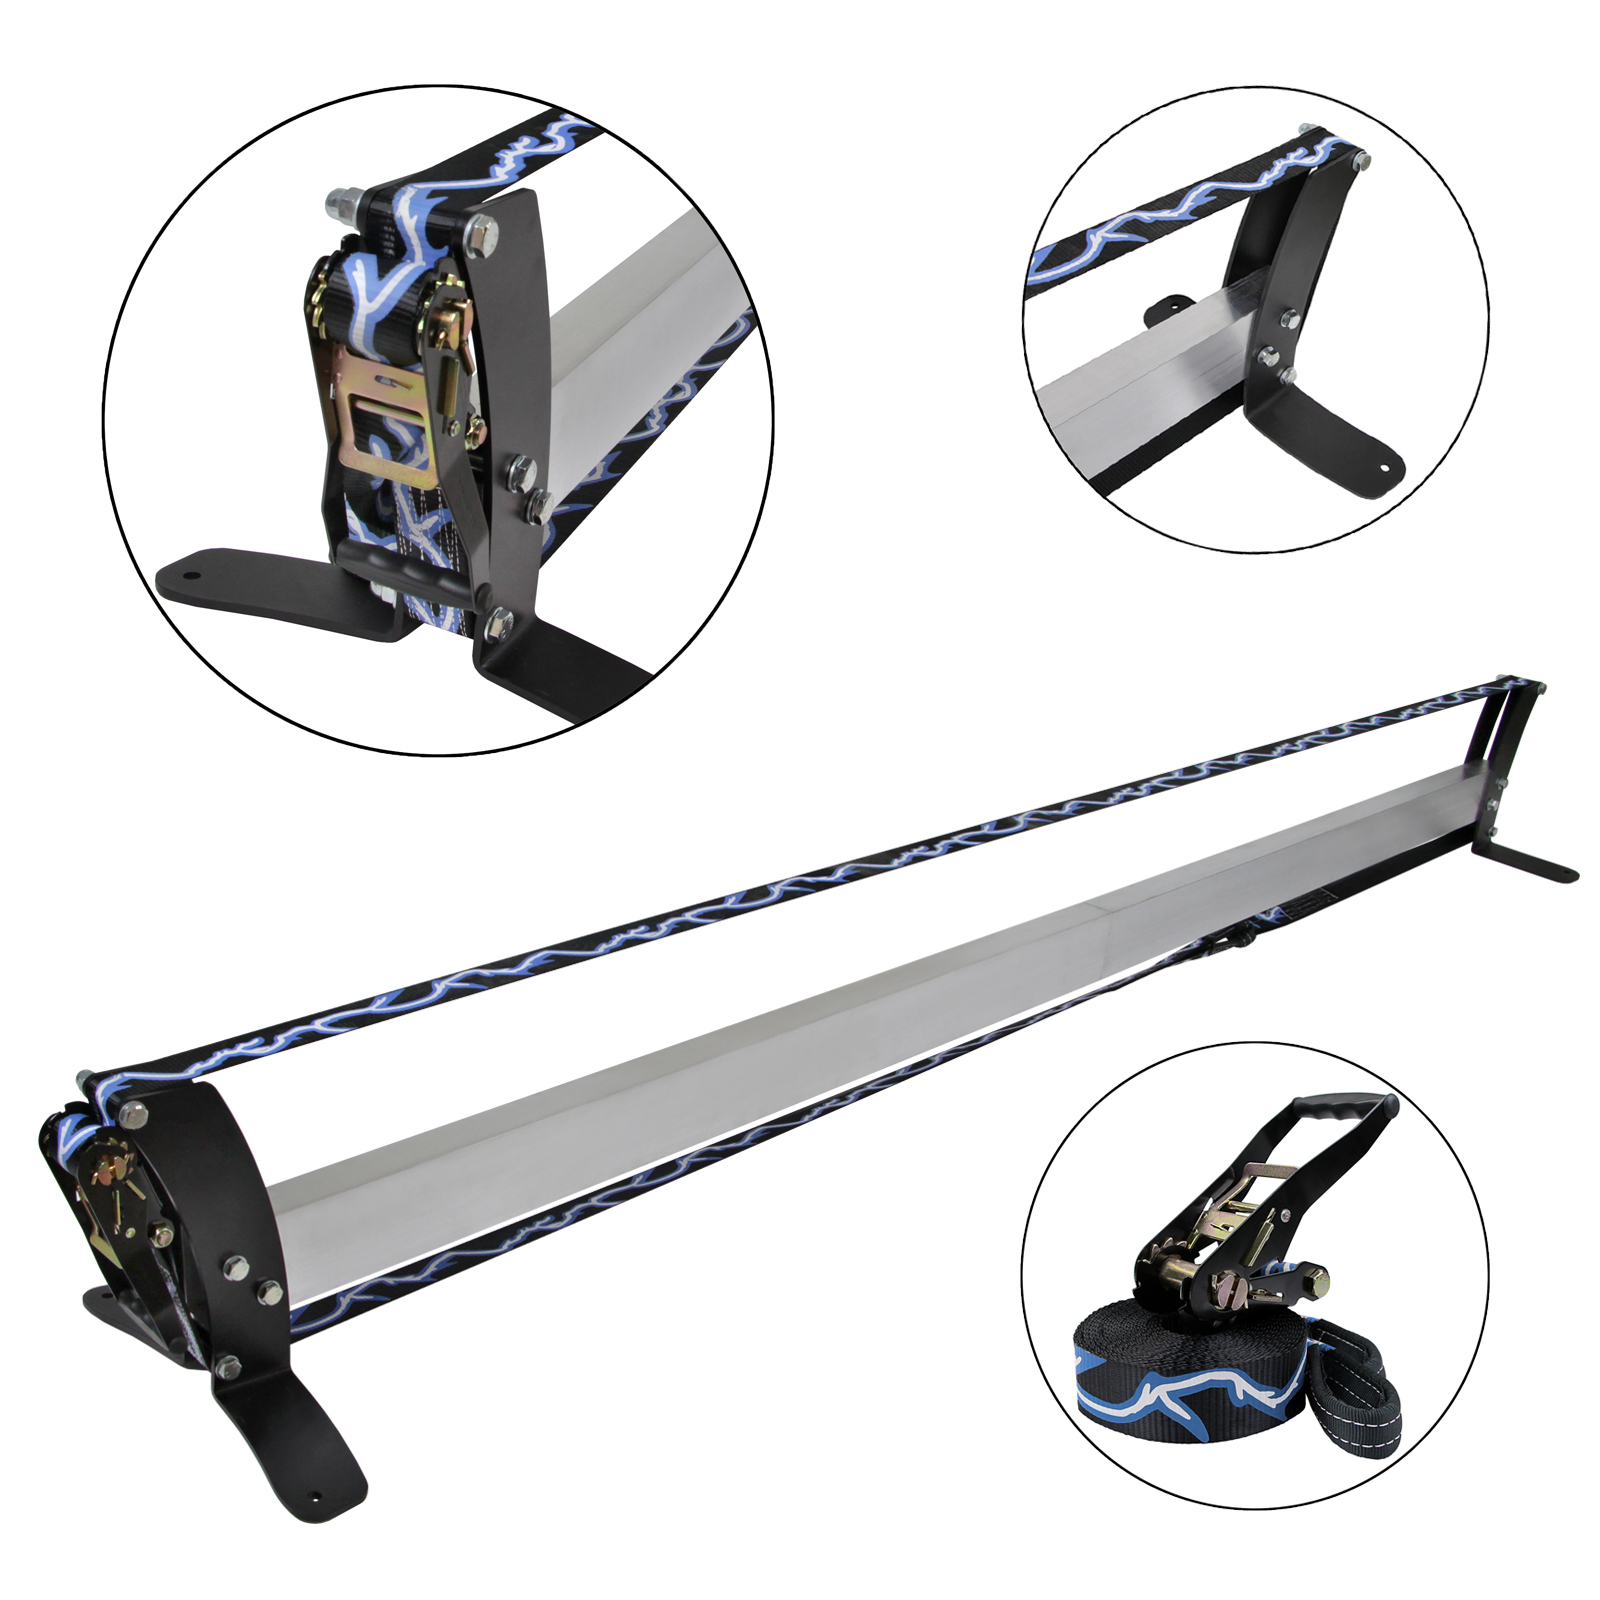
\includegraphics[width=0.4\linewidth]{Pictures/5_1_mobileSlackline}
		\caption{Mobile slackline \textit{alpidex POWER-WAVE 2.0}~\cite{alpidex2017-ms}}
		\label{fig:5_1_mobileSlackline}
	\end{minipage}
\end{figure}

It provides the needed mobility and independency due to its comparatively short length of three meters.
A major advantage is the possibility to set it up indoors as well as moving it in different positions with minimum effort.
The included slackline is tensed around brackets at both ends of the device.
%The middle rail is divided into two parts and needs to be put together.
It is placed in front of the \textit{Microsoft Kinect v2}, which is used as tracking device, like discussed in section~\textit{\nameref{trackingTechnologie}}.
The Kinect itself is attached on a tripod with a height of about 90 cm.
A \textit{STEAM® MACHINE by ZOTAC}~\footnote{Technical details of the STEAM® MACHINE: Intel Core i5-6400T @ 2.2 GHz, NVIDIA GeForce® GTX 960, 8 GB RAM} served as development PC that fulfilled the recommended specs of the Kinect.
%: \textit{Windows 8, 4 GB Memory, Physical dual-core processor with 3.1 GHz or faster, USB 3.0 Gen-2 controller, DirectX 11 Graphics card}.
As visual output device a projector with a resolution of 1920x1080 was attached on a traverse system.
The interface was visualized on a projector screen with a size of 2.40 x 3.00 m to give the user a more immersive feeling. A general overview about the interplay of all hardware can be seen in Figure~\ref{fig:5_3_systemArchitecture}.

\begin{figure}[htb]
	\centering
	\begin{minipage}[t]{0.58\linewidth}
		\centering
		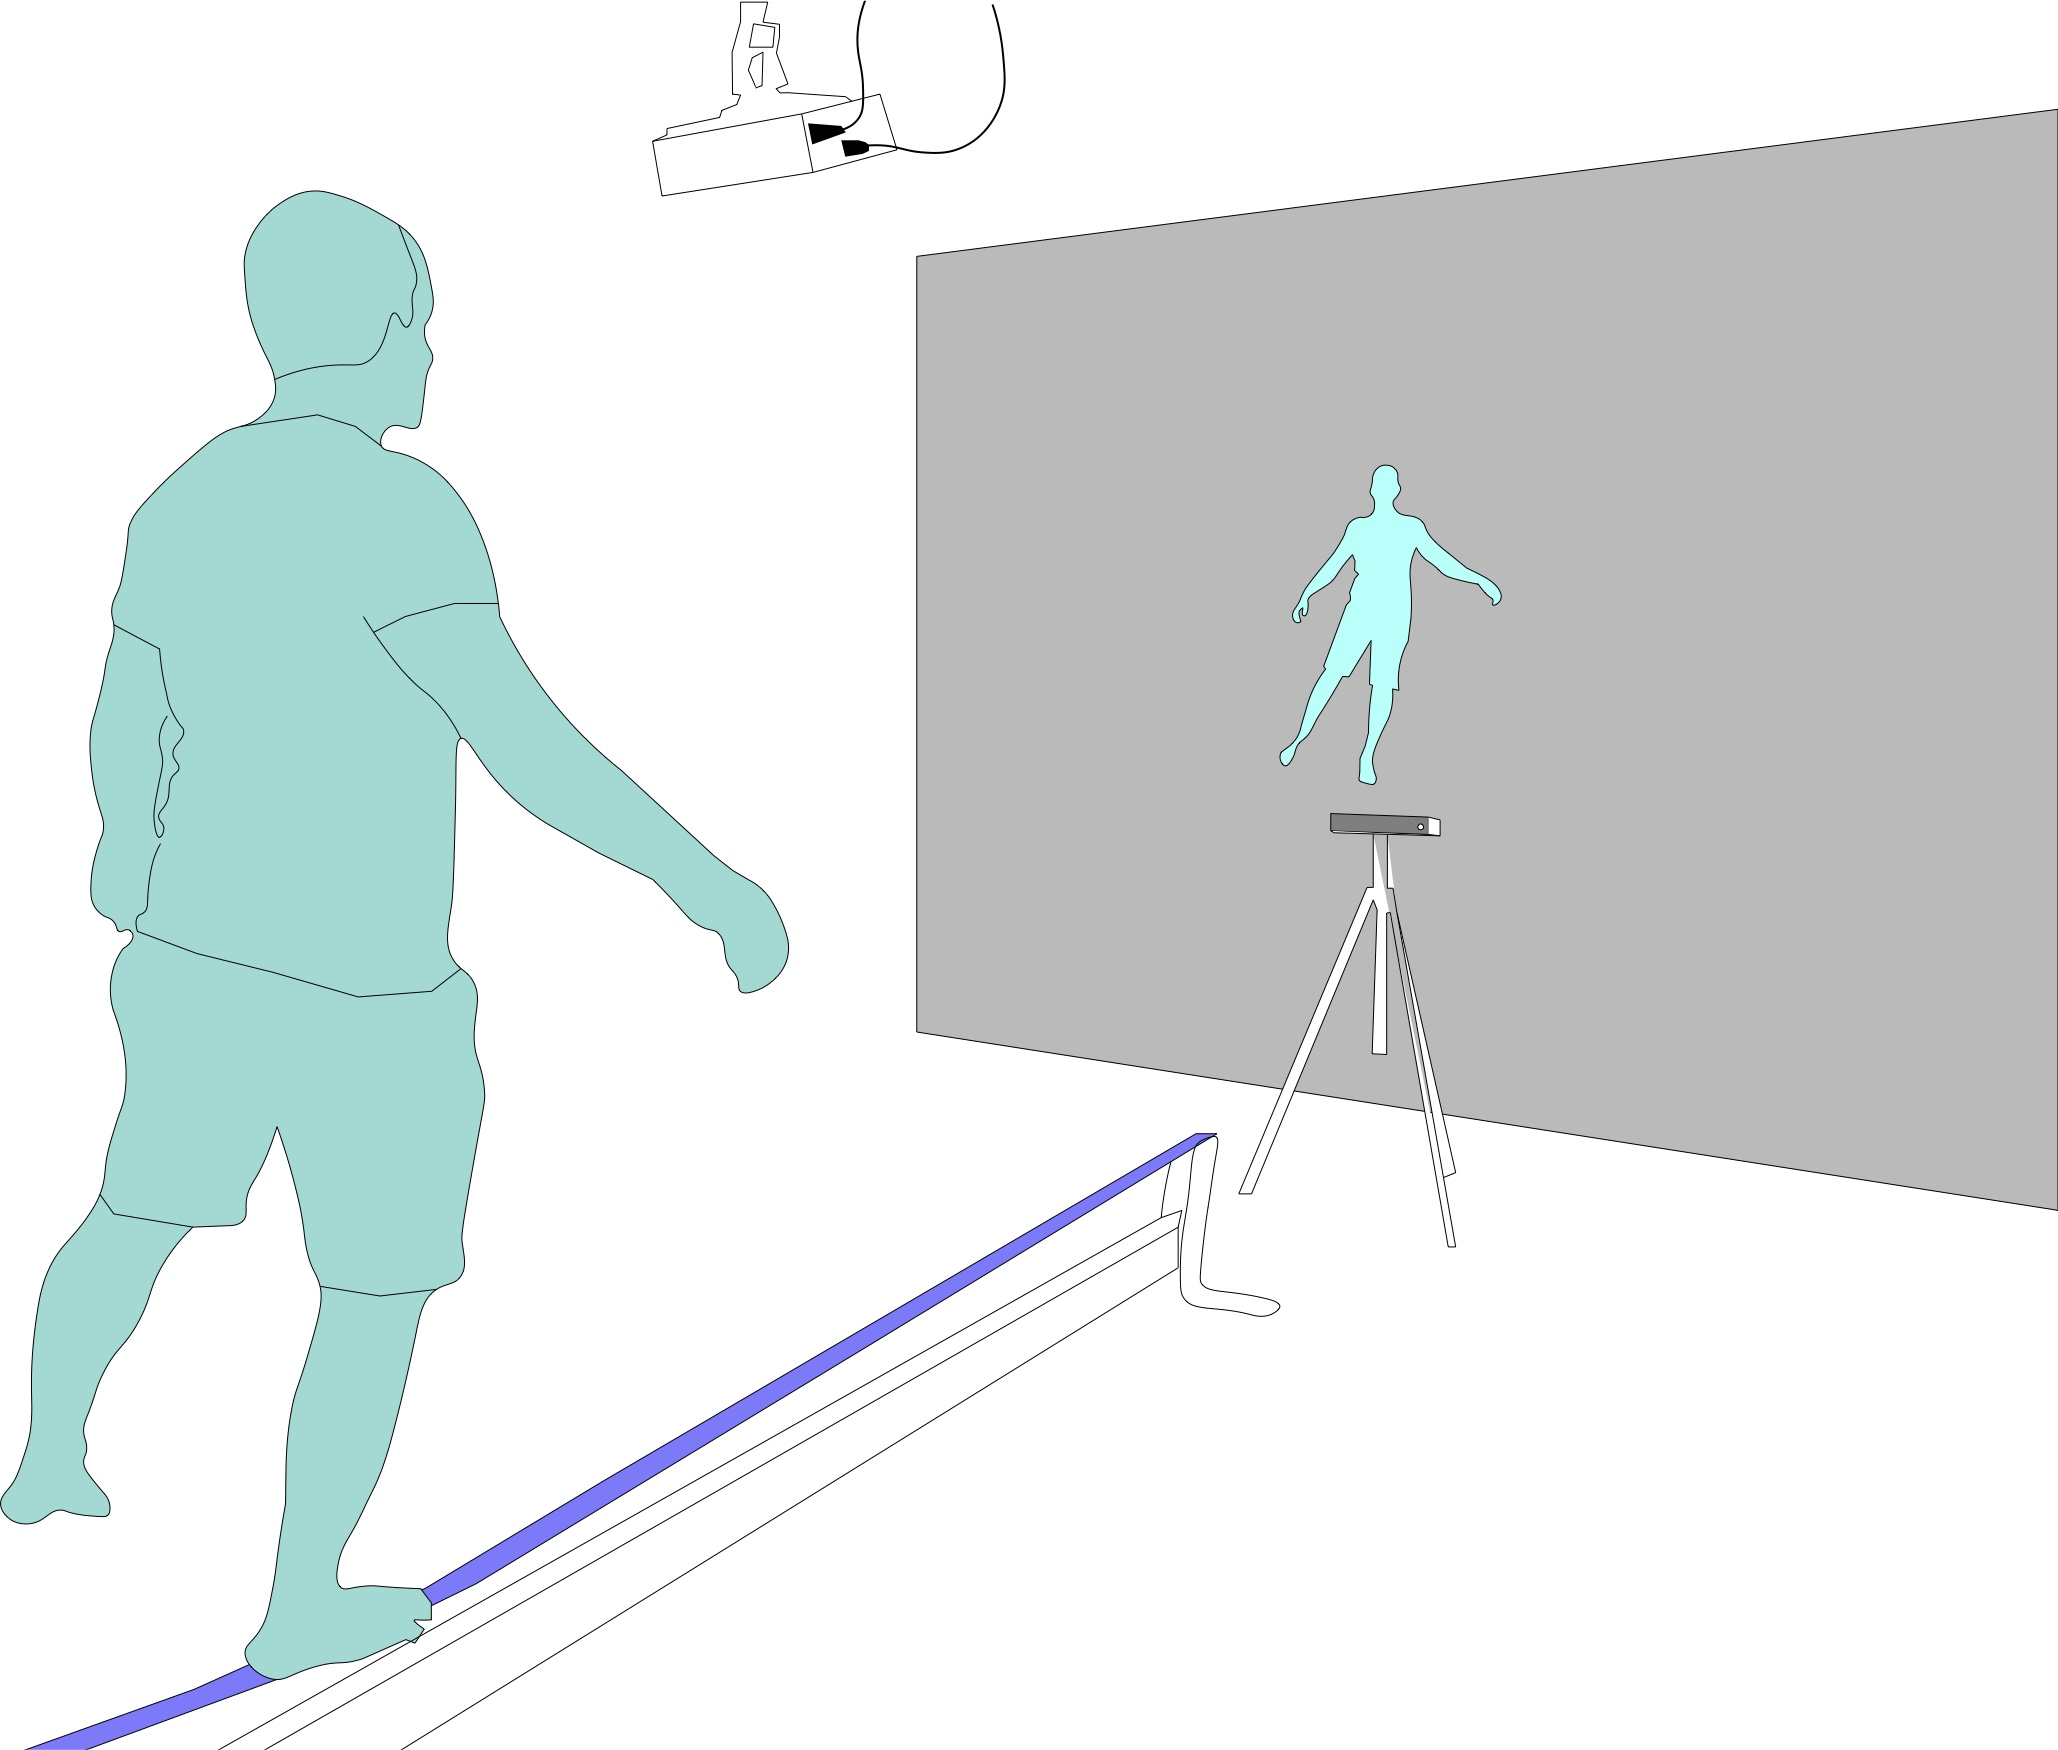
\includegraphics[width=1\linewidth]{Pictures/5_1_slackliner}
		\caption{Setup of all components}
		\label{fig:5_3_systemArchitecture}
	\end{minipage}
\end{figure}

\begin{comment}
\begin{figure}[htb]
	\centering
	\begin{minipage}[t]{1\linewidth}
		\centering
		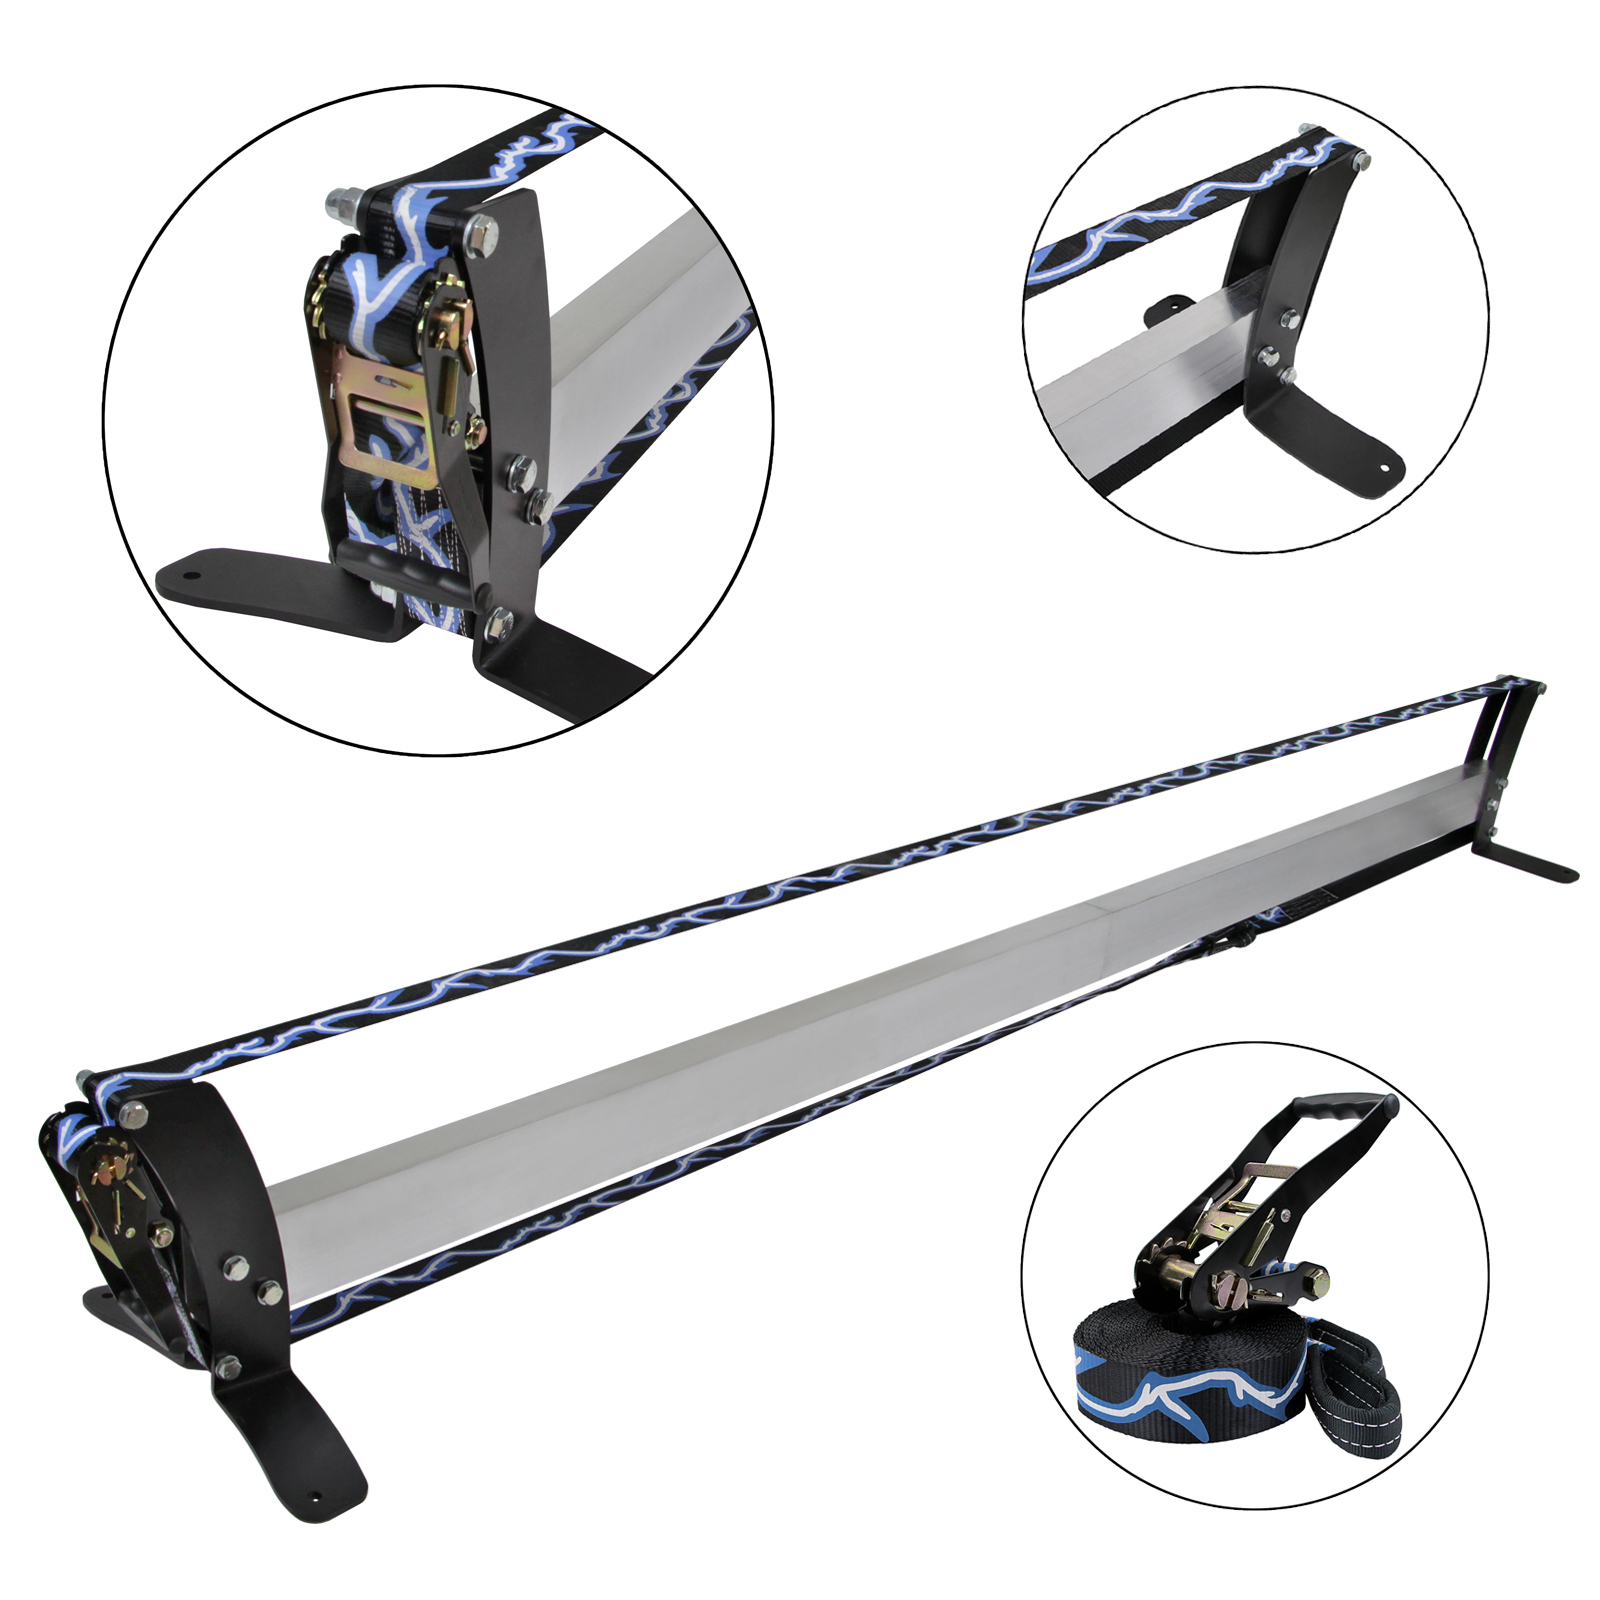
\includegraphics[width=0.44\linewidth]{Pictures/3_2_mobileSlackline}
		\caption{Mobile slackline \textit{alpidex POWER-WAVE 2.0}~\cite{alpidex2017-ms}}
		\label{fig:3_2_mobileSlackline}
	\end{minipage}
\end{figure}
\end{comment}

\subsection{Kinect and Slackline Positioning}\label{5_1_technicalFeasibility}
Tracking a person on a slackline with the Kinect is very different from the common use case.
The combination of the slackline range, vibration of the line, and unpredictable movements because of balancing actions of the user could lead to imprecise and inaccurate input data for tracking.
%disturb the tracking performance.
%Furthermore, no comparable work exist about how to track user appropriately on a slackine with the Kinect.
The major approach is to compare different slackline positions (Vertical: 0 Degrees, Diagonal: 45 Degrees, Orthogonal: 90 Degrees) regarding multiple angles and heights of the Kinect (80 cm, 160 cm, 240 cm), which is attached on a tripod or traverse system.
This scenario clarifies how good a person can be tracked on the entire slackline as well as at the beginning of the line for study purposes of this thesis.
%Moreover, which is the best combination of the slackline and Kinect positioning to track a user on the entire line as well as for study purposes of this thesis.
%The testing person was recorded via \textit{KinectStudio}~\footnote{\url{https://developer.microsoft.com/de-de/windows/kinect/tools}}, a tool for recording clips out of the streaming data of the Kinect.

\subsubsection{Limitations of the Kinect} 
A considerable role plays the angle and tracking range of the Kinects' depth sensor in the positioning.
Its angle of vision covers horizontally 70 degrees and vertically 60 degrees (see Figure~\ref{fig:5_1_1_visionAngle}).
Since the slackline is about 30 cm off the ground body parts of the user could be cropped depending on the Kinects' height and its angle.
The total tracking range of the sensor covers a range between 0.5 and 4.5 meters, whereas the sweet spot area lies between 1 and up to 4 meters (see Figure~\ref{fig:5_1_1_trackingRange})~\cite{MicrosoftHIG2014-mh}.
The mobile slackline device used in this thesis has a length of three meters and fits theoretically entirely within the sweet spot.
%it could lead to tracking problems by 
\begin{figure}[htb]
	\centering
	\begin{minipage}[t]{0.44\linewidth}
		\centering
		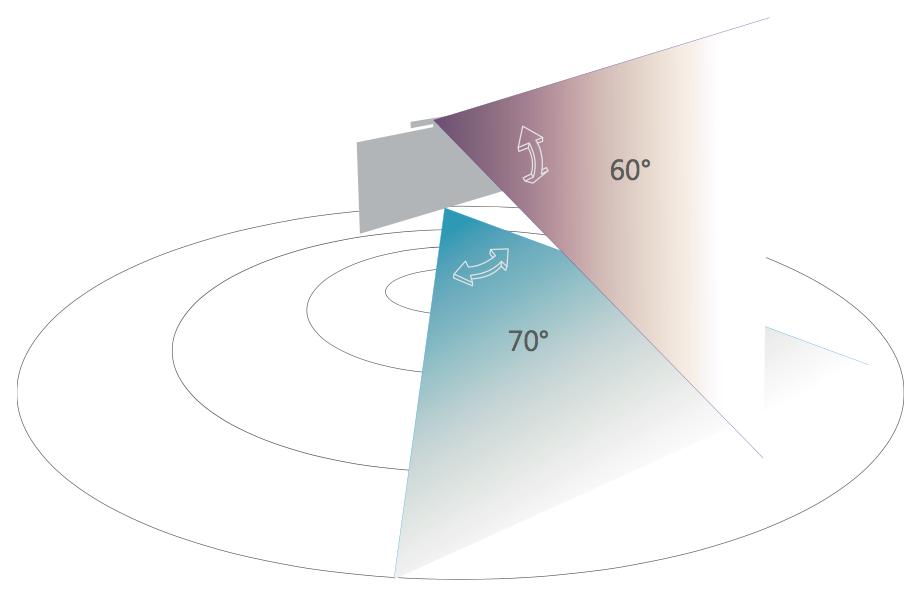
\includegraphics[width=1\linewidth]{Pictures/5_1_1_visionAngle}
		\subcaption{Angle of vision}
		\label{fig:5_1_1_visionAngle}
	\end{minipage}
	\hfill
	\begin{minipage}[t]{0.44\linewidth}
		\centering
		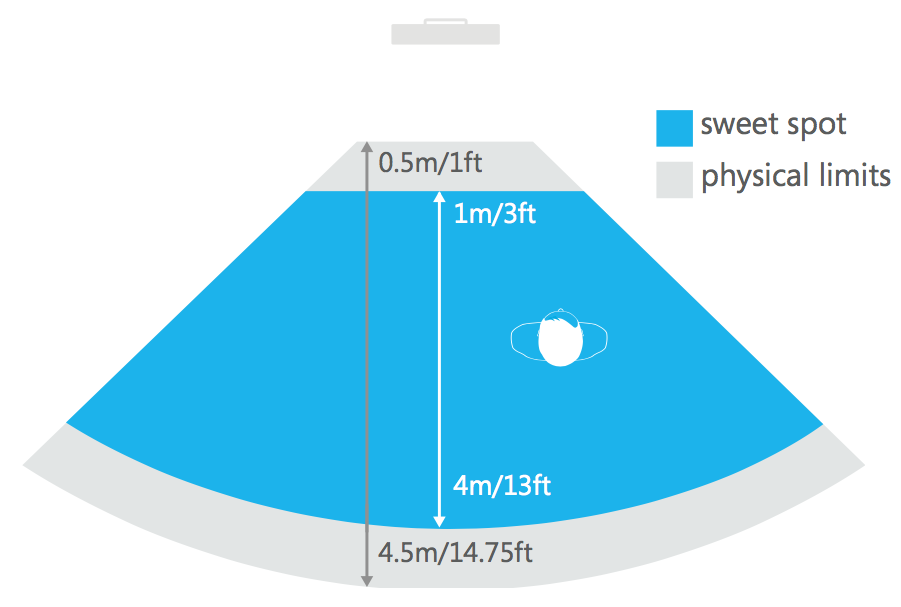
\includegraphics[width=1\linewidth]{Pictures/5_1_1_trackingRange}
		\subcaption{Kinect tracking range}
		\label{fig:5_1_1_trackingRange}
	\end{minipage}
	\caption{Limitations of the Kinect v2 sensor~\cite{MicrosoftHIG2014-mh}}
	\label{fig:5_1_1_sensorConstraints}
\end{figure}

%\subsubsection{Testing scenario}

%The test took place in the laboratory of the research group in the \textit{german reasearch center for artificial intelligence}~\footnote{\url{https://www.dfki.de/web/kontakt/dfki-saarbruecken}}. A big advantage of this is the large space to place the slackline easily in different variations. 
%The slackline is placed in three positions to the Kinect: frontal (0 Degree), diagonal (45 Degree) and sideways (90 Degree) \textbf{\todo{(Figure X - 1)}}. Each of this positions is tested regarding three different height levels of the Kinect: 80 cm, 160 cm, and 240 cm. Therefore it was attached on a tripod or traverse system (\textbf{\todo{Figure X - 2}}). At the end nine different combinations are covered to track a user on a slackline, which gives a general overview of the Kinect height to the slackline. The testing person was recorded via \textit{KinectStudio}~\footnote{\url{https://developer.microsoft.com/de-de/windows/kinect/tools}}, a tool for recording clips out of the streaming data of the Kinect.
%In the following the results discuss the feasibility and appropriate tracking positions.

\subsubsection{Best Positioning for Study Purposes}
\textbf{\textit{Slackline Positioning}}

With a slackline positioned orthogonal (90 Degrees) to the Kinect, no interference regarding the limit of the tracking range can happen because the whole body is in a constant line with the tracking area. However, permanent overlapping of body parts resulted in problems to detect body joints with an appropriate accuracy and precision (see Figure~\ref{fig:5_3_slacklineSideways}).
When placing the slackline diagonal (45 Degrees) the body is more visible to the sensor and showed better results.
%to the Kinect several body parts will not overlap.
%the frontal and end point of the slackline now differ in the vertical axis, which is unproblematic  \textbf{\todo{(Table X and Figure X)}}. 
%This could even result in a better trackability in matter of the depth field range, since the distance in the front shrinked and is therefore closer to the Kinect depth view. 
Tracking failure still happen especially when regaining equilibrium on the line. Mainly the joints of the arms and legs interfere with other body joints (see Figure~\ref{fig:5_3_slacklineDiagonal}).
In addition, every time the user wants to interact with the Kinect she has to turn towards it, which leads to a more complicated user experience.
%which makes it also unusable.
%This results in a relatively bad skeletal tracking and depending on the executed exercise it can lead to detection problems.
Positioning the slackline vertical to the Kinect avoids this. Furthermore, the sensors' view can see the full body and track joints without any occlusion.
Problems occurred at the starting position of the slackline since it uses the entire tracking range.
The user stands here at the outermost limit of this range, where the detection of the Kinect begins to get worse (see Figure~\ref{fig:5_3_slacklineVertical}).
Because of this the slackline must be arranged, such that the starting position of the line lies within the sweet spot area.
%Because of this the slackline must be positioned close to the Kinect for study purposes.
%The starting position of the line is now within the sweet spot area of the Kinect tracking range.
%Three main height levels were used to show the main differences of the tracking behaviour from the Kinect. It is mounted on a tripod and covers the heights of 0.80, 1.60 and 2.40 meters off the ground.
\begin{figure}[htb]
	\centering
	\begin{minipage}[t]{0.32\linewidth}
		\centering
		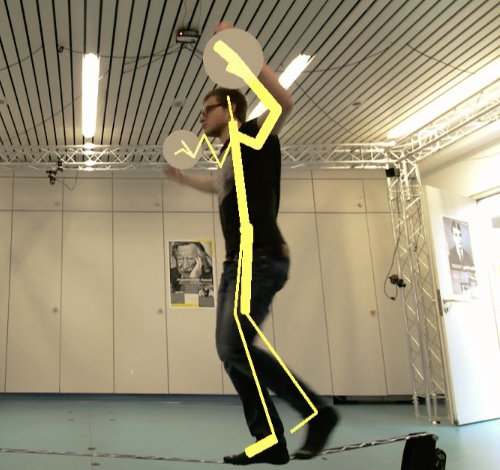
\includegraphics[width=1\linewidth]{Pictures/5_3_slacklineSideways}
		\subcaption{Sideways}
		\label{fig:5_3_slacklineSideways}
	\end{minipage}
	\hfill
	\begin{minipage}[t]{0.32\linewidth}
		\centering
		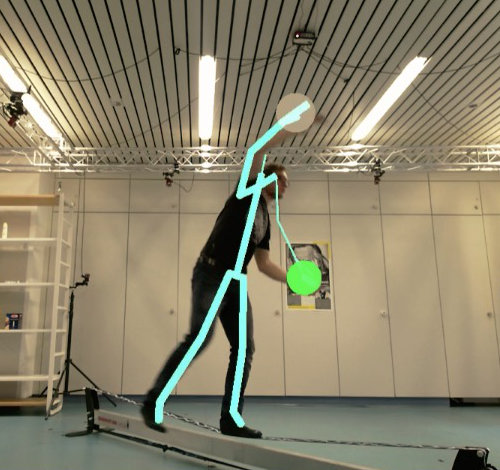
\includegraphics[width=1\linewidth]{Pictures/5_3_slacklineDiagonal}
		\subcaption{Diagonal}
		\label{fig:5_3_slacklineDiagonal}
	\end{minipage}
	\hfill
	\begin{minipage}[t]{0.32\linewidth}
		\centering
		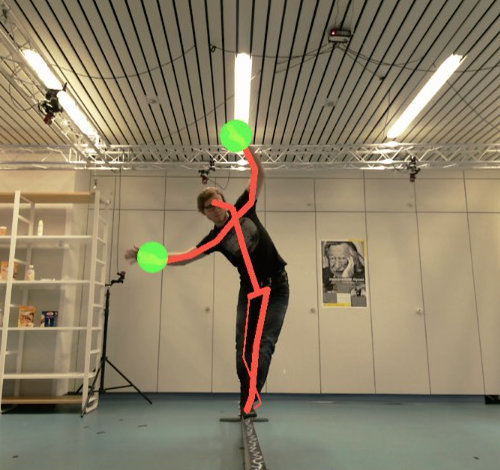
\includegraphics[width=1\linewidth]{Pictures/5_3_slacklineVertical}
		\subcaption{Vertical}
		\label{fig:5_3_slacklineVertical}
	\end{minipage}
	\caption{Different positions of the slackline. The coloured lines visualise the skeletal tracking of the Kinect. Thin lines represents inferred joints}
	\label{fig:5_3_slacklinePositionings}
\end{figure}

\textbf{\textit{Kinect Height}}

Beginning with a height of 2.40 meters the Kinect has a very steep view angle.
%to track the slackers' body on the full range of the slackline. 
Hereby, the tracking range shifts more downwards and shrinks in its height (see Figure~\ref{fig:5_3_kinectHeightHigh}).
With users of a height above 1.85 m the starting position cannot be arranged for appropriate usage.
%If beginning at the starting position on the slackline the slacker reaches hereby immediately the end of the tracking area. 
The same problem applies for a Kinect height of 1.60 m. The view angle is more flat but the slackline must be positioned further away from the Kinect to prevent cropped body parts like the head or arms (see Figure~\ref{fig:5_3_kinectHeightMiddle}).
%Also the further she walks towards the Kinect the more joints of the feet overlap.
%With a height between 1.60 and 1.20 meters the view angle is more flat but the slackline must be positioned further away from the Kinect to prevent cropped body parts like the head or arms (Figure\ref{fig:5_3_kinectHeightMiddle}).
A height of 1.20 up to 0.80 meters results in a flatter view angle and therefore in a more homogeneous view and tracking range (see Figure~\ref{fig:5_3_kinectHeightLow}).
The body is fully visible in the entire tracking range and not limited in the height of the Kinect view.
Additionally the Kinect is in a position that won't disturb the visual sense of the slacker during her training on the slackline, e.g. by setting a focus point in front of her.
%Problems can occur with positioning the Kinect on a lower height. It can lead to cropped body parts like the head or arms at the very end of the slackline.

\begin{figure}[htb]
	\centering
	\begin{minipage}[t]{0.32\linewidth}
		\centering
		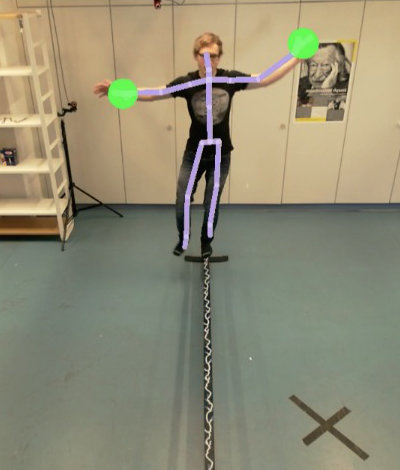
\includegraphics[width=1\linewidth]{Pictures/5_3_kinectHeightHigh}
		\subcaption{Kinect height of 2.40 m}
		\label{fig:5_3_kinectHeightHigh}
	\end{minipage}
	\hfill
	\begin{minipage}[t]{0.32\linewidth}
		\centering
		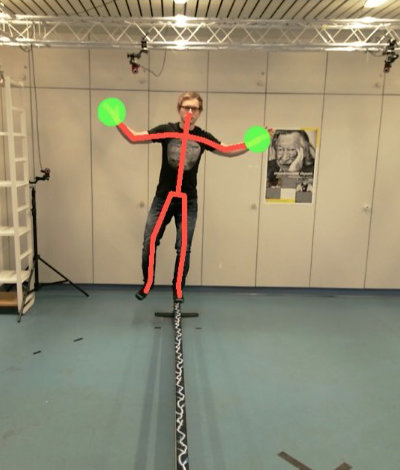
\includegraphics[width=1\linewidth]{Pictures/5_3_kinectHeightMiddle}
		\subcaption{Kinect height of 1.60 m}
		\label{fig:5_3_kinectHeightMiddle}
	\end{minipage}
	\hfill
	\begin{minipage}[t]{0.32\linewidth}
		\centering
		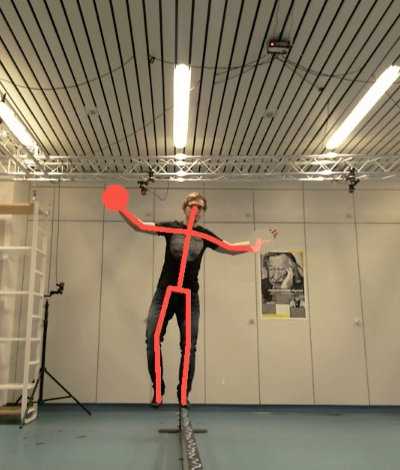
\includegraphics[width=1\linewidth]{Pictures/5_3_kinectHeightLow}
		\subcaption{Kinect height of 0.80 m}
		\label{fig:5_3_kinectHeightLow}
	\end{minipage}
	\caption{Kinect view on different heights. The coloured lines visualises skeletal tracking.}
	\label{fig:5_3_kinectHeights}
\end{figure}

%The tracking and view is more homogeneous and the angle flatter, which results in the possibility to use the full depth range. With a higher attachment the angle will be too steep, which results in less depth range, as well as more occlusions of body parts can occur.
\begin{comment}
\rowcolors{2}{tablerowgray}{tablerowgray}
\begin{table}[h!]
\centering
%\arrayrulecolor{white}
\renewcommand{\arraystretch}{1}
\begin{tabular}{| c c c | c c | c c c |}
\hline
\rowcolor{tableheadergray} & \multicolumn{7}{| c |}{\textbf{Slackline Positioning (m)}} \\ 
\rowcolor{tableheadergray} \textbf{Kinect Height (m)} & \multicolumn{2}{ c |}{\textbf{Vertical}} & \multicolumn{2}{| c |}{\textbf{Diagonal}} & \multicolumn{3}{ c |}{\textbf{Sideways}}\\
\rowcolor{tableheadergray} & \textbf{Front} & \textbf{Back} & \textbf{Front} & \textbf{Back} & \textbf{Front} & \textbf{Back} & \textbf{Mid} \\
\hline
2,40 & 1.30 & 4.30 & 1.90 & 3.80 & 3.00 & 3.00 & 2.70 \\
\hline
1.60 & 1.70 & 4.70 & 2.10 & 4.00 & 3.00 & 3.00 & 2.70 \\
\hline
0.80 & 1.30 & 4.30 & 1.90 & 3.80 & 2.60 & 2.60 & 2.10 \\
\hline
\rowcolor{green} 0.80 - 1.20 & 0.00 & 4.00 & - & - & - & - & - \\
\hline
\end{tabular}
\caption{Combination of Kinect height and slackline positioning}
\label{table:1}
\end{table}
\end{comment}

% But since beginner will use the entire slackline range it can be neglected.
The best combination resulted in placing the slackline vertically and having a Kinect height of 0.80 up to 1.20 meters. Hereby, the Kinect can track the entire body with nearly no joint overlap.
Since the focus of the study in this thesis lies mainly on beginners, the starting position of the slackline is important and must not lie at the outermost tracking range.
Hence, it makes more sense to move the slackline very close to the Kinect. The starting position on the line fits then within the sweet spot area.
%a higher tracking confidence is possible.
%plays an important role and 
%because the very end of the line is not necessary for the study.
%a little bit of slackline is cropped out of the view but 
%A higher tracking confidence is possible at the starting position, which is more important in this case \textbf{\todo{(Figure X)}}.
%This results in a relatively bad skeletal tracking and depending on the executed exercise it can lead to detection problems.
\section{Data Model}\label{5_2_dataModel}
All relevant data are stored in JSON files. It is more human-readable and makes accessing as well as updating data simple. Each user should have the same basis of exercises. A default exercise JSON file serves as template for all registered users in the SLS. An internal editor was created to make data management and adjustments more easy. Figure~\ref{fig:5_2_dataModel} shows the overall data structure.

A user data file represents the profile of a slacker who wants to train with the system. It consists of her name and a default template of levels and exercises. Only one user profile at a time can be active. This ensures that no other profiles can affected by the current user.

\begin{comment}
A level can be unlocked and accomplished, e.g. at the beginning the very first level is unlocked but not accomplished since no exercise has been finished.
Further, it consists of a level name that will be displayed to the slacker and a file name for loading the appropriate gesture database.
The specific goals and a description list are included.
Several exercises can be part of a level.
\end{comment}

A level has a name, can be unlocked, and accomplished. Unlocking the next level means the current one has been successfully accomplished. This again means that each exercise of it has been finished. Furthermore, each level consists of a name, a list of goals, and a description that gives hints about the general execution of its exercises.
Several exercises are part of a level.


\begin{comment}
Exercises can also be unlocked, accomplished and have an exercise name to be displayed. In addition they have a file name to load the appropriate exercise in the database, pictures for a preview in the , and videos in the application. For the gesture detection it is important to store if the current exercise is discrete or progress gesture. The purpose of this is further described in Section~\textit{\nameref{5_3_movementRecognition}}. Further, the average user time, average confidence, and entire amount of attempts out of both sides for this exercise are stored. Lastly, each exercise has two sides.
\end{comment}

Exercises consists of a name and a thumbnail picture that is shown in the menu. A description and a looping video of the correct execution are provided in the introduction.
For each body side the user has to challenge several repetitions with a minimum time to hold the specific position.
If all repetitions have been successfully executed for both body sides, the current exercise is accomplished and the next one will unlock.
A check list provides the user during her training with supportive real-time feedback, which guides her for a successful exercise execution.
%looks after specific movements that the user has to do for the correct execution.
The users' performance of the current execution is given by a constant varying confidence value. If her movement exceeds a certain confidence, a timer starts and she has to hold the exercise until a predefined minimum time has been reached.
%an exercise is executed with a certain confidence the time that runs 
%The time the user needed to execute the exercise, the confidence she achieved by matching the pre-defined exercise in the database, and the amount of attempts are stored. 
%These parameter provide post-feedback about her performance progress of the exercise. They are also used to analyse the difficulty level and progress for each user in the study.
An exercise has a type that can be either discrete or continuous, which is important to know for the user tracking. 
The actual exercise is stored as a gesture in the database to match it against the current user movement.
The next Section~\textit{\nameref{5_3_movementRecognition}} describes the purpose of a type, gesture, and the database more specifically.

\begin{comment}
Every side can be accomplished and unlocked. A direction specifies the current side, which can be either left or right. The actual exercise description is also stored here, as well as the average user time, average confidence, and the entire attempts out of all repetitions.

Multiple repetitions are part of a side. A single repetition consists of a minimum time the user has to reach, the time of the user in execution, her confidence, and the amount of attempts she needed. 
Further the side has a checklist, which is used to help the user for the correct exercise execution.
\end{comment}

\begin{figure}[htb]
	\centering
	\begin{minipage}[t]{1\linewidth}
		\centering
		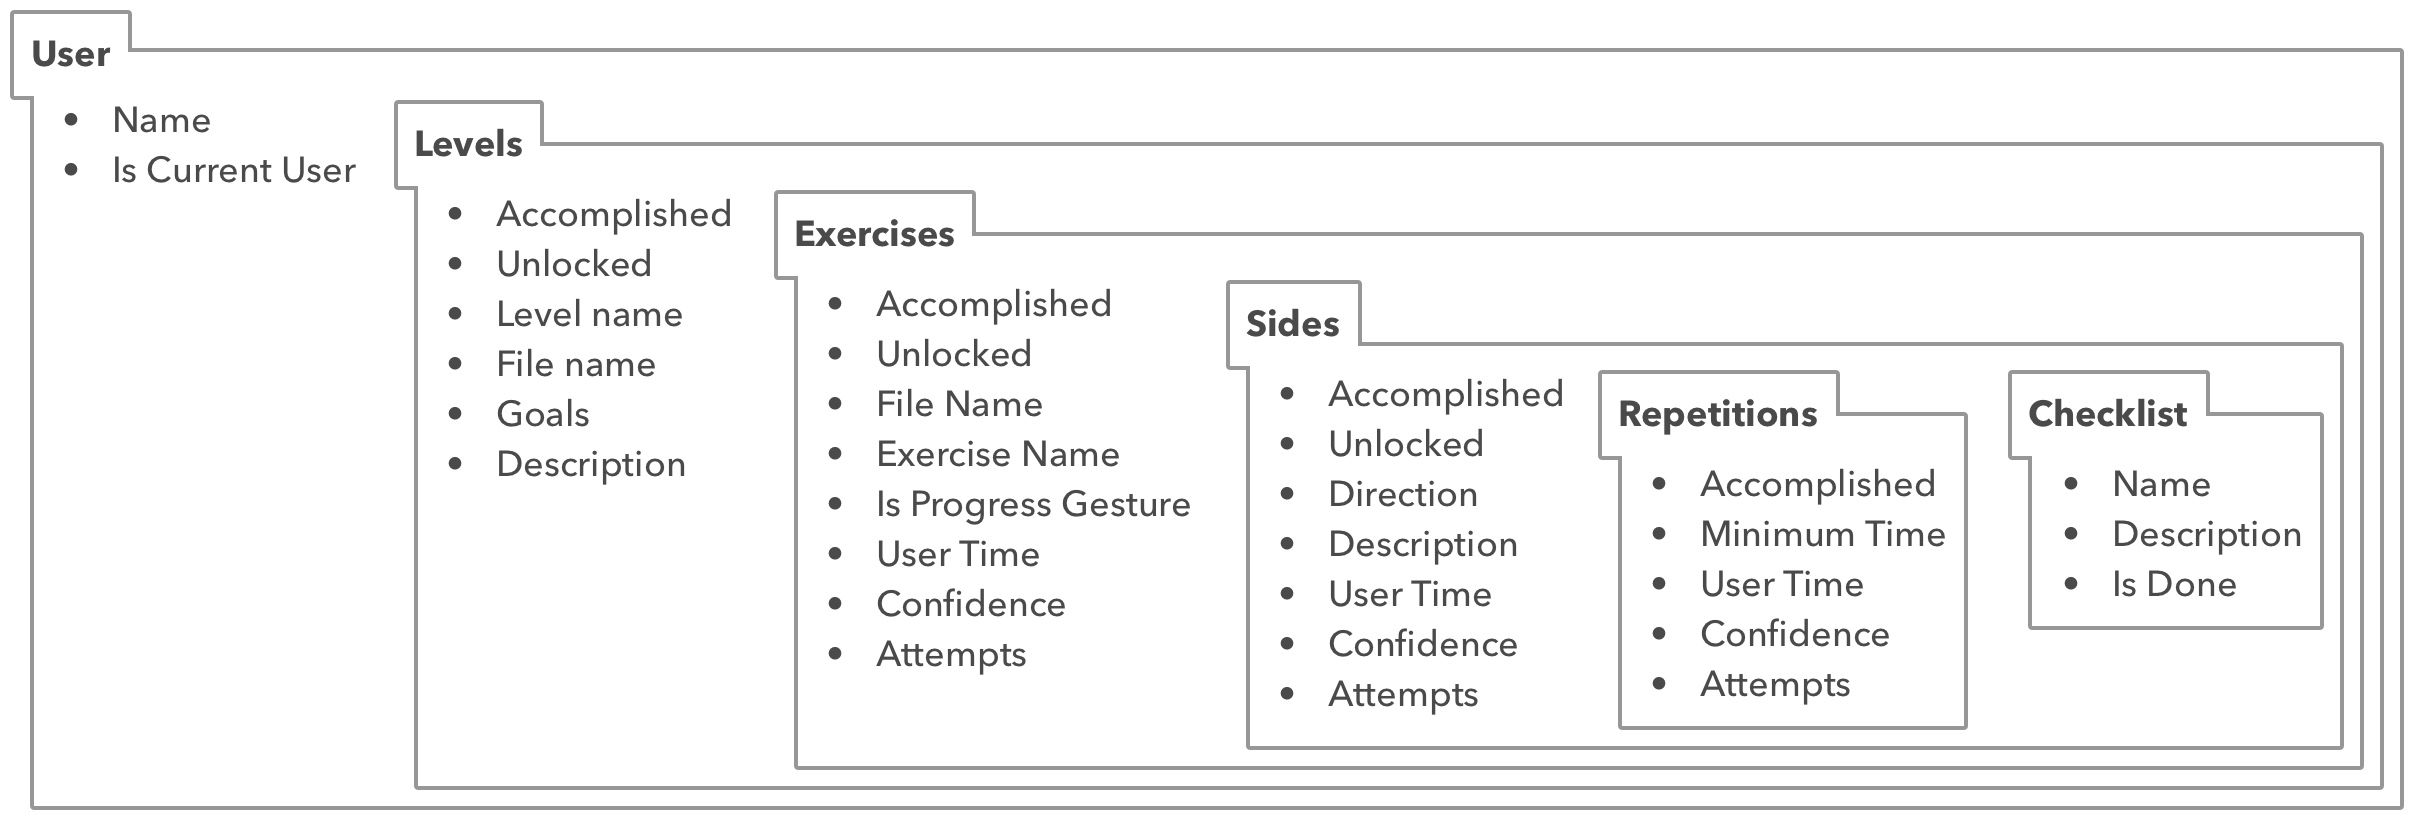
\includegraphics[width=1\linewidth]{Pictures/5_2_dataModel}
		\caption{Data model overview}
		\label{fig:5_2_dataModel}
	\end{minipage}
\end{figure}

%- Name, Side
%-- Side, Description, Min time, Repetitions
%-- Average user time, user attempts, confidence
%-- Checklist
%--- Repetitions
%--- User time, User time, Attempts
%- Average user time, user attempts, confidence
%- Gesture

%This application a 3D project has been generated, since the Kinect uses 3D space to track the user, she should be able to interact within that, and a 3-Dimensional environment design is considered. Further some examples of the interaction implementation is described.

%For each object containing key-value pairs a class is generated, i.e. for Users, Tier, Exercise, Sides, and Repetitions. In listing \todo{ref c\# code example} an example for the \textit{Tier} object can be seen. A class must be marked as serializable to work with the JSON serializer. It contains variables, which match the JSON structure on listing \todo{ref json code}. 
%\todo{c\# code example and json file}

%With this an instance of the class can be created and the value accessed for adjustments (listing \todo{ref img class instance}). This can then be serialized into a JSON object. Line \todo{ln number} shows how existing JSON data can be converted back into an object instance. This is needed to fetch user data that already exists.

%The files are stored within the \textit{StreamingAssets} folder of Unity. Data stored in this folder can easily be accessed via path name of the target machines file system. 

\section{Movement Recognition}\label{5_3_movementRecognition}
%- Recording of gestures --> Kinectstudio --> Making/Train gestures --> Visual gestures builder
The SLS guides the trainee through predefined exercises for slacklining. In the case of this thesis it is important to know that exercises are defined as \textit{gestures} within the context of the Kinect development. The \textit{Kinect for Windows Human Interface Guidelines} describe the term gesture as follows: "\textit{[...] we use the term gesture broadly to mean any form of movement that can be used as an input or interaction to control or influence an application.}"~\cite{MicrosoftHIG2014-mh}.

\subsection{Heuristics vs. Visual Gesture Builder}
The Kinect SDK provides two approaches for tracking a gesture in an application~\cite{MicrosoftVGB}.
The first one is called heuristic approach, which means to manually track each body joint position of the user in the code.
Conditions can be defined according to the action that should happen e.g. if a joint exceeds a certain threshold or is in a defined range.
Heuristics are mainly used for simple gestures like raising the hand over the head, which is implemented in the SLS as engagement gesture.
For more complex gestures, the developer must have a good understanding about the movement and behaviour of the human body.
Furthermore, environmental factors like an inappropriate mounting of the Kinect could exacerbate managing and maintaining the code.

Usually a common developer has not the appropriate expertise of the human body behaviour or it would take too much effort.
Hence, it is recommended to use the Visual gesture builder (VGB) provided by Microsoft. 
More complex gestures can be easily defined. For example doing one legged squats is a sequence of multiple actions with several factors (It is also implemented in the SLS as an exercise).
The VGB uses machine learning to build a database out of pre-recorded clips.
Afterwards it can be implemented in an application to track the desired gesture.
A major advantage is that environmental factors are not as complex to handle as in comparison to heuristics.
The user just records multiple clips with the Kinect and builds a new database.
In the heuristic approach this has to be considered manually in the code.
The cons of the VGB are the huge file size of the recorded clips that can take very much disk space.
Also tagging the clips for the gestures, which should be detected by the application, is time consuming. 
On the other hand the tool is simple to use and constructing complex gestures can be easy like described in the next subsection.


%any form of movement that can be used as an input or interaction to control or influence an application. Gestures can take many forms, from simply using your hand to target something on the screen, to specific, learned patterns of movement, to long stretches of continuous movement using the whole body.

\begin{comment}
\subsection{Visual gesture builder}
%look at the data given by the developer via pre recorded clips.
%The more data is provided to the database, the better the detection. konkretisieren
%The VGB uses machine learning to build a database out of pre-recorded clips by the developer.
%Afterwards the database can be implemented in an application to track the defined gesture.
A major advantage is that environmental factors are not as complex to handle as in comparison to heuristics.
For example if the application should cover that the Kinect can be mounted in an inappropriate height, the developer has to consider this in his heuristics.
Managing and maintaining such factors in code can be demanding.

With the VGB the developer just records data with the Kinect in the appropriate height and let the machine learning algorithm learn it.
The cons are the huge file size of the recorded clips which can take very much disk space.
Also tagging keyframes for recorded clips, which should be detected by the application is time consuming. 
On the other hand the tool is simple to use and constructing complex gestures can be easy like described in the next subsection.
\end{comment}

\begin{comment}
\subsection{Categories of indicators}
An indicator defines the machine learning technology with which the gesture will be learned.
It can be categorized in a discrete or continuous gesture.
Discrete gestures underlay a conditional check in which the application determines if a certain gesture is currently performed or not.
It provides a confidence value that compares the correctness of the persons execution regarding the gestures in the database.
This is the majority usage for gesture tracking like e.g. raising the hand or lifting a leg.

A continuous gesture however means that a progress can be measured instead of the confidence.
Usually a sequence of motions is combined to an entire gesture.
The progress gives feedback about the ongoing movement of the person regarding the gesture.
This could be for example a golf swing or switching the standing leg~\cite{MicrosoftVGB}.
\end{comment}

\subsection{Workflow for Building Gestures}
The workflow for creating a gesture follows a general routine (Figure~\ref{fig:5_3_gestureCreation}).
At first the gesture has to be recorded via \textit{KinectStudio}.
This is a tool provided by Microsoft for monitoring and recording raw clips of the Kinect streams.
Before inserting the clip into the VGB a new project has to be created.
Therefore, the developer first selects the body parts that are necessary for the gesture.
After that an indicator has to be defined, which can be either discrete or continuous.
Discrete gestures define a binary state and validates if a certain gesture is currently performed or not (e.g. standing on one leg).
It provides a confidence value that compares the correctness of the persons execution regarding the gestures in the database.
A continuous gesture means usually the combination of motions to a sequence of small gestures (e.g. switching standing leg).
Instead of the confidence, a progress value gives feedback about the ongoing movement of the person matching the gesture sequence in the database.

After the project creation the recordings can be inserted as training data.
The developer has to tag the clips to define a starting as well as an end point of the gesture.
After finishing with tagging a database file can be built.
It is recommended to test it via a live preview or with other recorded clips in a separate analysis area.
If the results are not satisfying, more clips can be recorded and added as training data or existing tags of the clips can be adjusted.
After the testing phase the gesture database file is ready for the integration in the application to detect gestures in runtime. %The structuring of the application architecture is part of the next section.
\begin{figure}[htb]
	\centering
	\begin{minipage}[t]{1\linewidth}
		\centering
		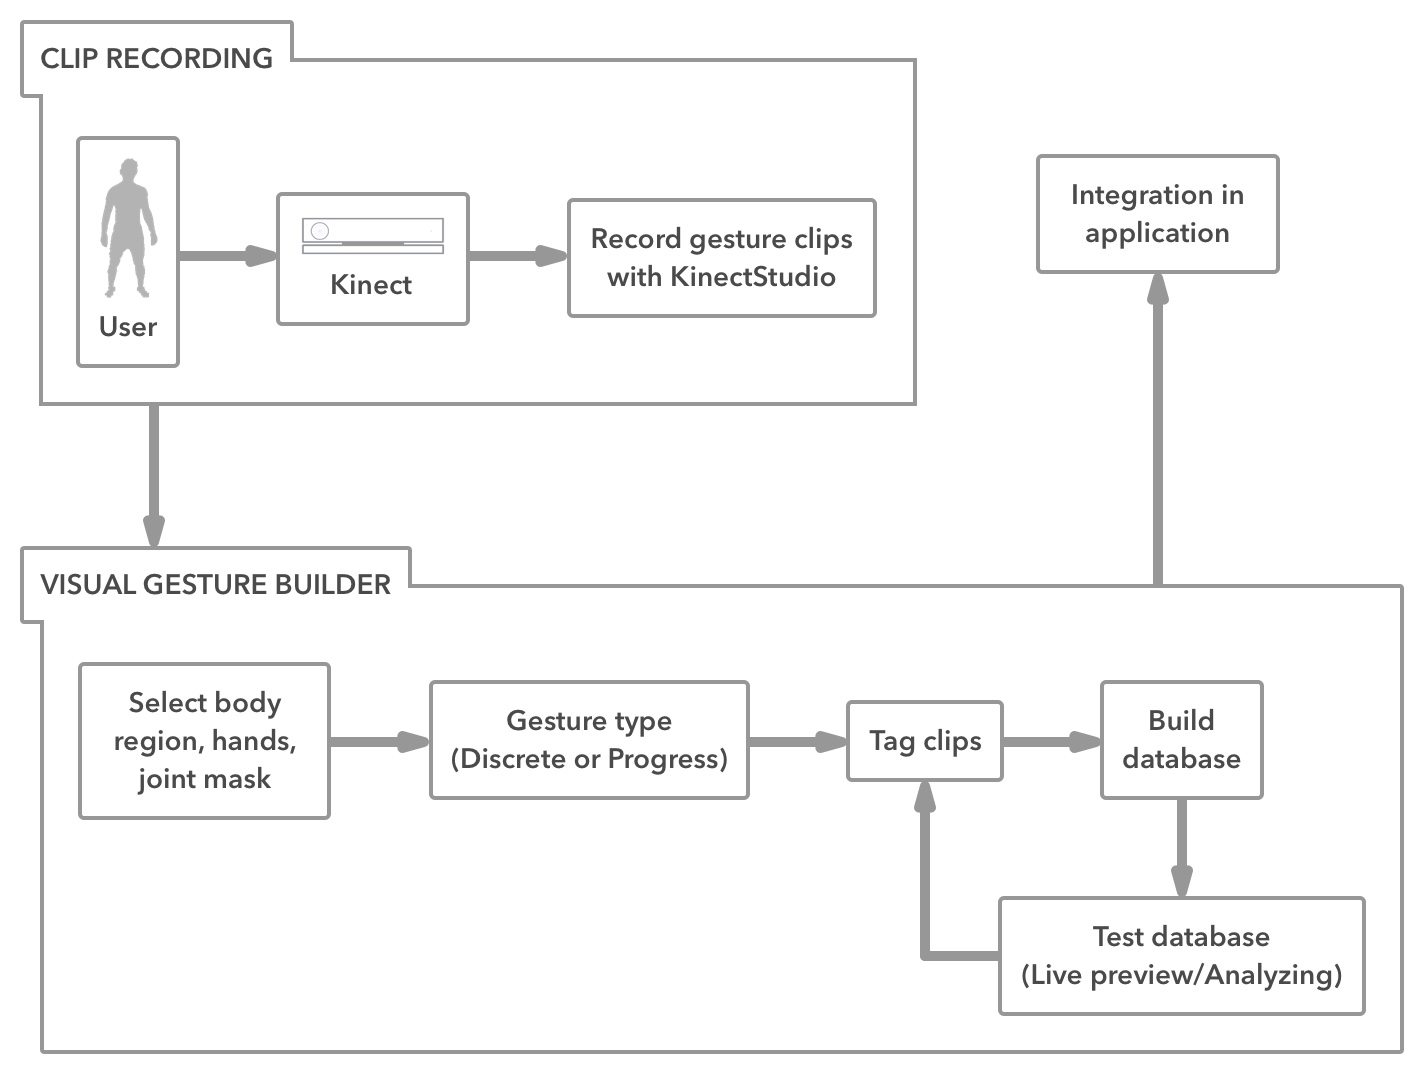
\includegraphics[width=1\linewidth]{Pictures/5_3_gestureCreation}
		\caption{Workflow of creating a gesture database}
		\label{fig:5_3_gestureCreation}
	\end{minipage}
\end{figure}
\section{Frontend}\label{5_4_software}
\subsection{Unity3D and Kinect SDK}
% KinectStudio, VGB, Unity3D, Kinect SDK for unity, Kinect MS-SDK
The software development process consists of the interplay of two major software components (Figure~\ref{fig:5_3_unityKinectArchitecture}).
First the cross-platform game engine \textit{Unity3D} by \textit{Unity Technologies}. It is widely known for game development but also for development with several interaction devices (e.g. \textit{HTC Vive}, \textit{Leap Motion}). Applications can be deployed for various platforms like desktop, mobile, web, console, TV, or virtual/augmented/mixed reality devices.
Unity is used in the SLS to create the virtual environment, interface design, manage actions by the user, and for data management.
%(e.g. Windows, macOS, Android, iOS, Oculus Rift, Windows Mixed Reality and so on).
\begin{figure}[htb]
	\centering
	\begin{minipage}[t]{1\linewidth}
		\centering
		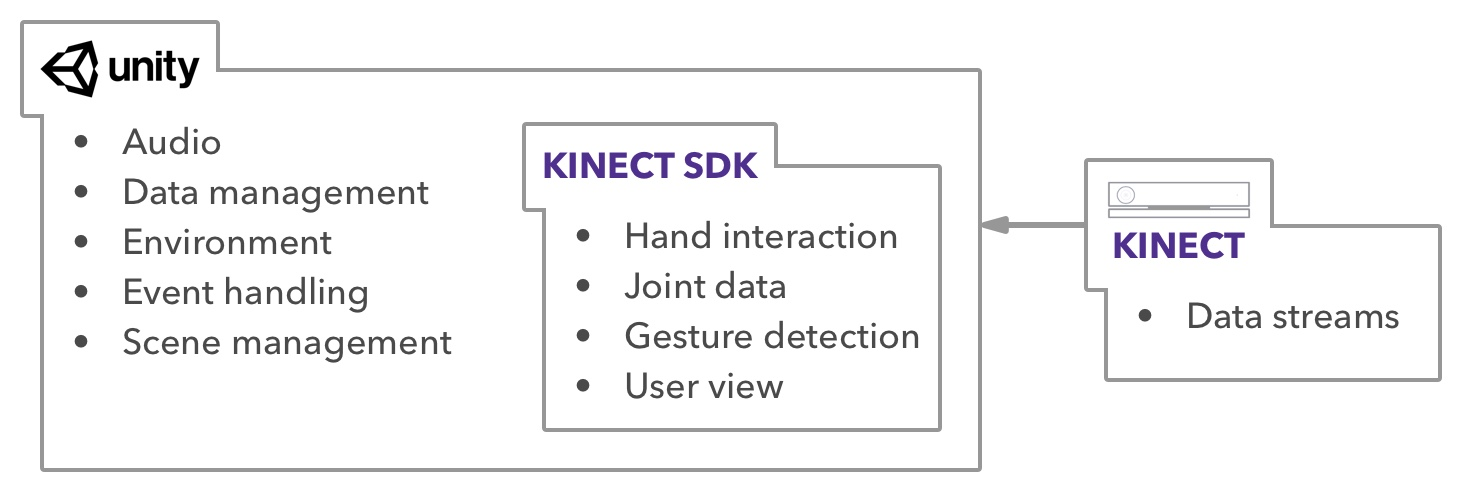
\includegraphics[width=1\linewidth]{Pictures/5_3_unityKinectArchitecture}
		\caption{Unity and Kinect architecture}%
		\label{fig:5_3_unityKinectArchitecture}
	\end{minipage}
\end{figure}

As second component the \textit{Microsoft Kinect SDK v2.0}~\footnote{\label{fn:kinectTools}\url{https://developer.microsoft.com/de-de/windows/kinect/tools}} has to be installed on the PC as well.
It consists of several tools, application examples, and scripts to access the data stream of the Kinect.
Microsoft offers also a \textit{Kinect for Windows Unity package}\cref{fn:kinectTools} to create a Kinect based Unity application.
%Since \textit{Unity 5} it can be used with the free personal edition of Unity, whereas before it could be only used with the pro version.
The \textit{Kinect v2 Examples with MS-SDK} \footnote{\url{https://www.assetstore.unity3d.com/en/\#!/content/18708}} package by Rumen Filkov was used to get an idea on how to handle the data streams of the Kinect.
In addition it makes accessing input data of the user recognized by the Kinect, like e.g. joint position and interaction implementation, more simple and provides several code examples.

%make data access and interaction implementation more simple as well as 
%The plugin is used for accessing input data of the user recognized by the Kinect device like e.g. joint position, gesture detection, and user actions.

%The JSON datafiles can be easily accessed in Unity via the JSON serialization feature~\footnote{\url{https://docs.unity3d.com/Manual/JSONSerialization.html}}. \todo{1-2 sätze mehr dazu}

\subsection{Implementation}
The frontend implementation of the SLS will be explained on the basis of the workflow that a user would run through. It consists of four main parts. First a small tutorial to get familiar with the interaction,  second the selection menus, third the description and introduction of a level as well as an exercise, and fourth the exercise execution with real-time feedback. 
%interaction integration, and feedback implementation of the system are further described.

\subsubsection{Interaction Tutorial}
If a user starts with the SLS (Figure~\ref{fig:5_3_welcome}) an engagement gesture is the very first interaction. She has to raise any hand over the head. This conveys that the system recognises and reacts to specific movement actions. 

Afterwards the user is introduced into the interaction techniques (Figure~\ref{fig:5_3_tutHandPush} \&~\ref{fig:5_3_tutHandPoint} ).
Her hands serve hereby as input for navigating and interacting with interface elements in the SLS. Therefore she is in constant interaction with the system and becomes more familiar to it.
The current position on the screen is visualised by a virtual hand cursor.

\begin{figure}[htb]
	\centering
	\begin{minipage}[t]{0.32\linewidth}
		\centering
		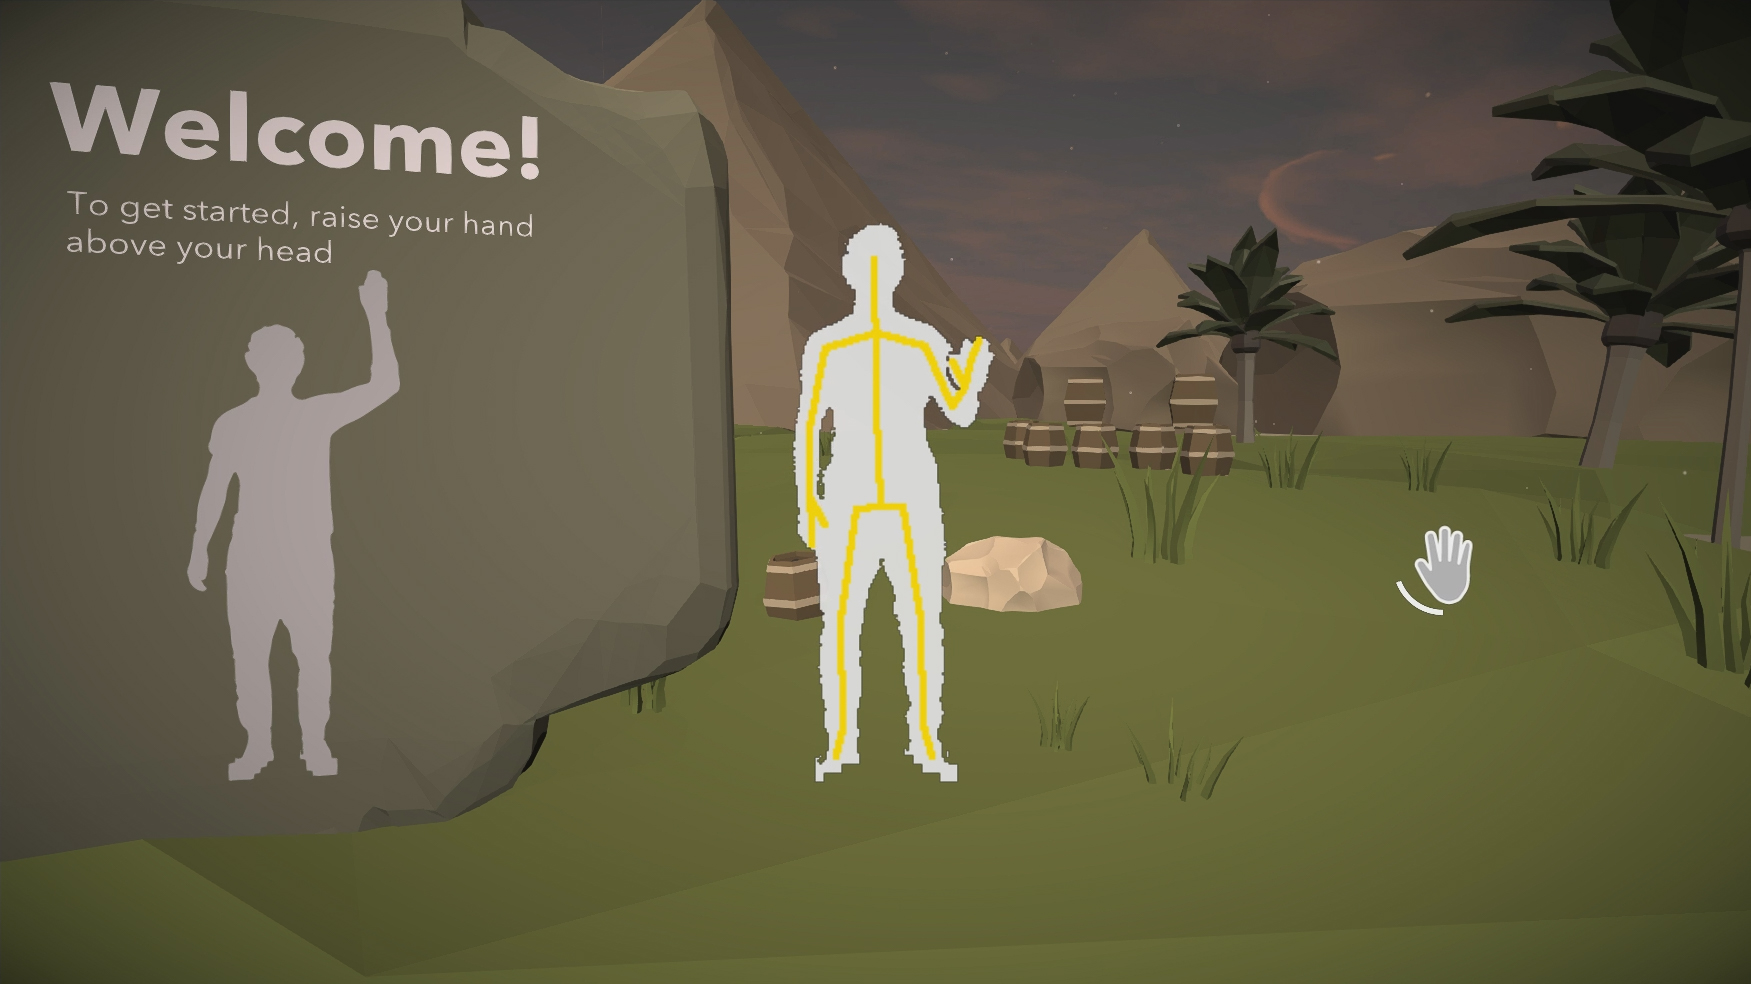
\includegraphics[width=1\linewidth]{Pictures/5_Workflow/1_Welcome}
		\subcaption{Welcome screen with engagement gesture}
		\label{fig:5_3_welcome}
	\end{minipage}
	\hfill
	\begin{minipage}[t]{0.32\linewidth}
		\centering
		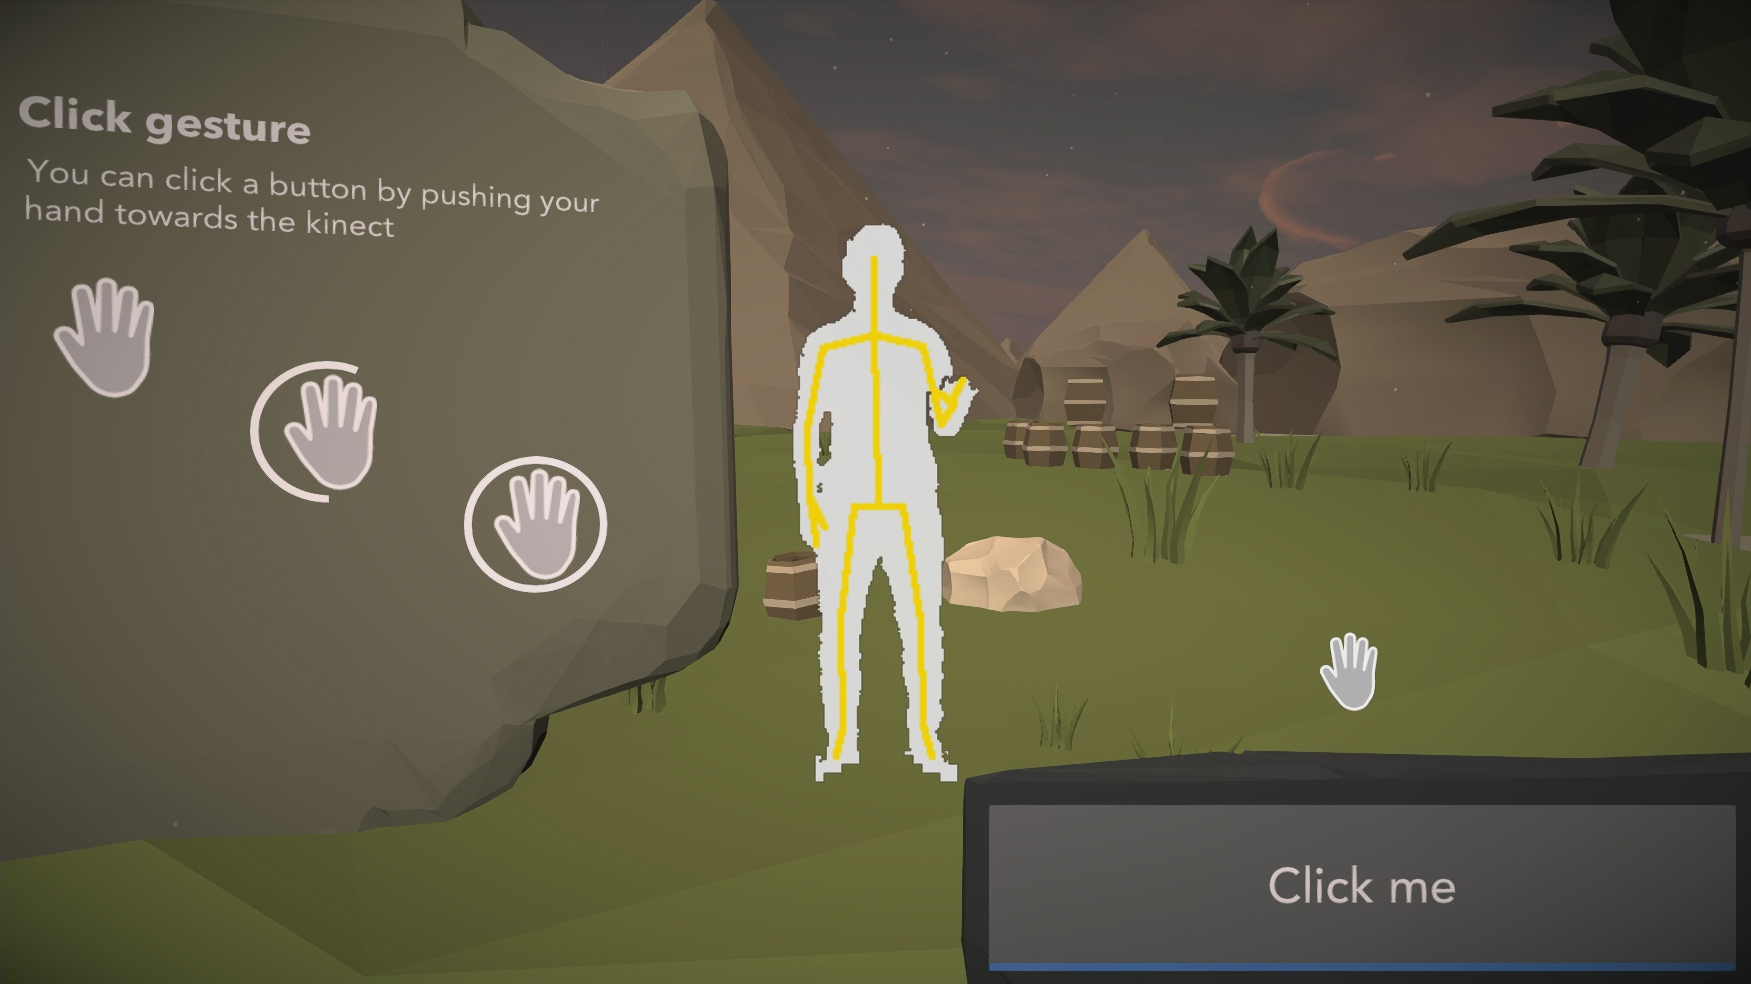
\includegraphics[width=1\linewidth]{Pictures/5_Workflow/2_TutHandPush}
		\subcaption{How to click part I}
		\label{fig:5_3_tutHandPush}
	\end{minipage}
	\hfill
	\begin{minipage}[t]{0.32\linewidth}
		\centering
		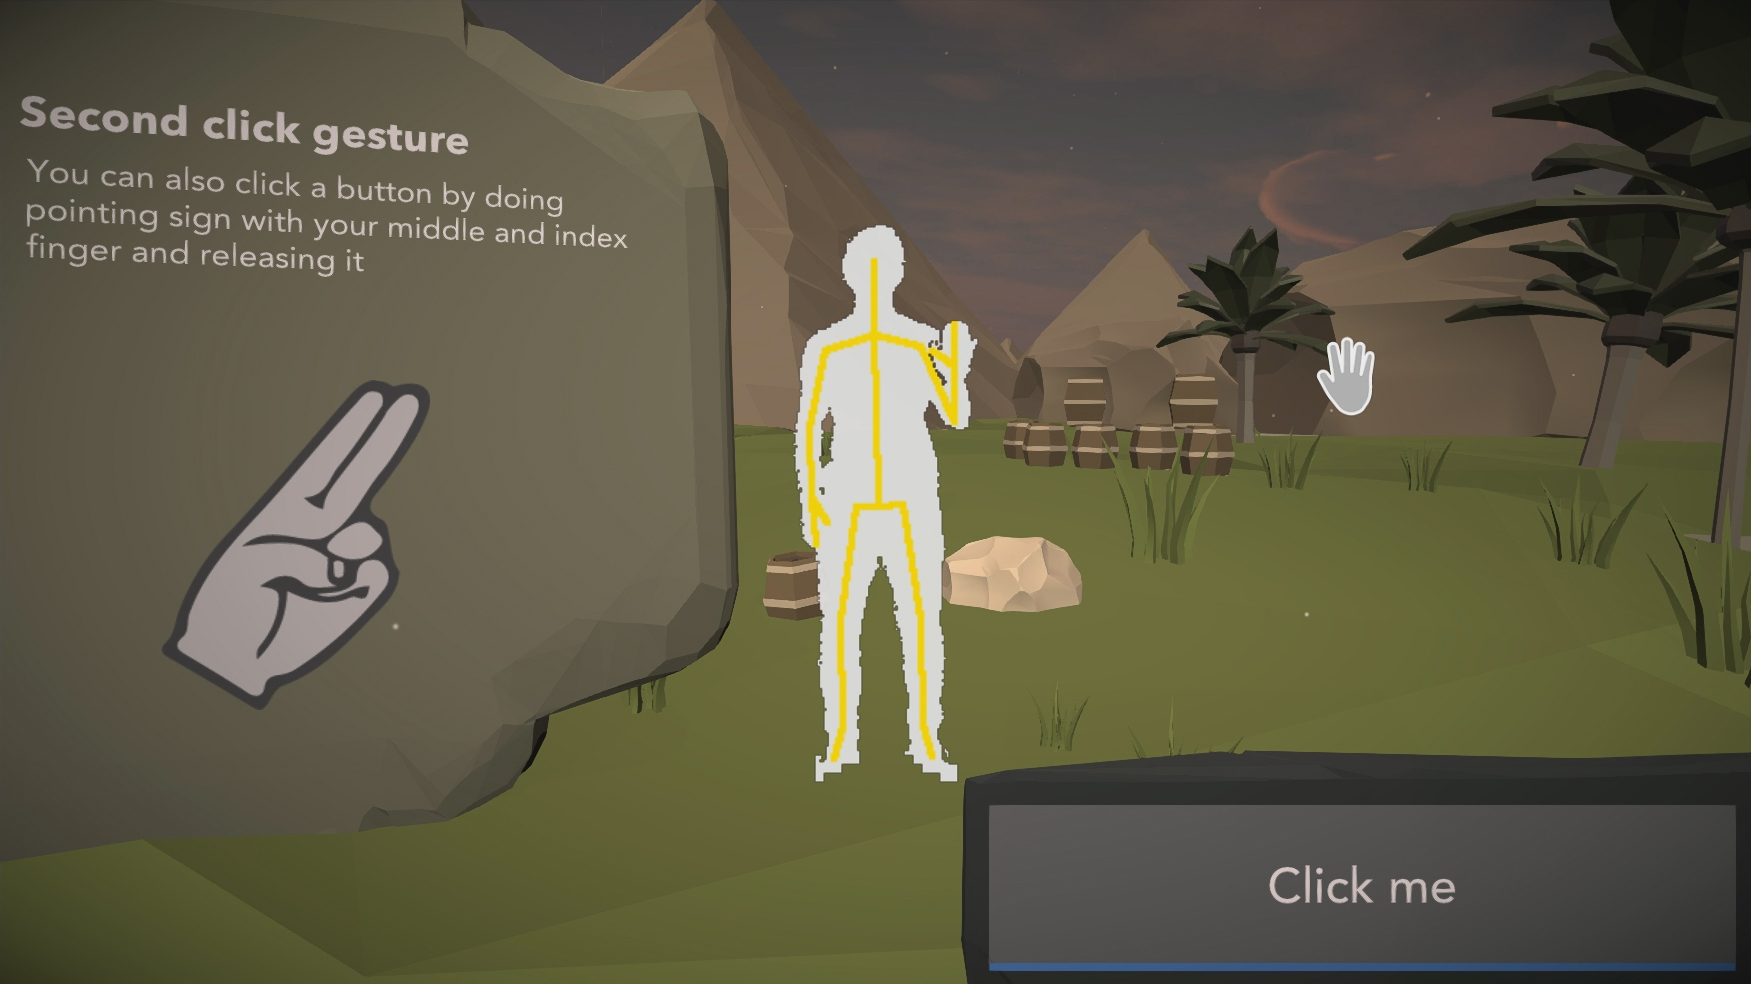
\includegraphics[width=1\linewidth]{Pictures/5_Workflow/3_TutHandClick}
		\subcaption{How to click part II}
		\label{fig:5_3_tutHandPoint}
	\end{minipage}
	\caption{Instruction on how to use the SLS}
	\label{fig:5_3_tutorials}
\end{figure}
%She has to raise her hand over the head whereupon the system conveys that it recognises specific user actions.

%A code example on how to this gesture is implemented can be seen in listing~\ref{lst:codeEngagement}.

%The \textit{KinectManager} exists as an empty \textit{GameObject} in the scene and has to be referenced in the script. The \textit{KienctInterop} class delivers several utility and interop function and calls the sensor interfaces. Here it is used to assign the proper joint type for tracking them. 
%First the developer has to assure that the Kinect is initialized, a user has been detected, and the relating joints are recognized. A condition checks if the current vertical position of the right hand is above the head joint (\textit{Listin~\ref{lst:codeEngagement} line~\ref{lst:codeEngagement15}}). If this is the case, the next scene can be loaded. 
%This is actually part of the script for the first scene in the application, in which the user has to engage with the Kinect by doing the described movement.

% provide the possibility of an autonomous interaction the user has to navigate on her own with the system.
%Her hands serve as input for interacting with interface elements.

Four different approaches were tested as hand interaction gesture.
First, hovering with the hand over elements for a few seconds (Figure~\ref{fig:5_3_hover}).
It caused problems because of accidental and unwanted misclicks due to relatively big and many interaction elements in the interface.
As second interaction technique the hand should be closed to a fist or grab gesture (Figure~\ref{fig:5_3_fist}).
It also triggered unwanted misclicks if the hand of the user closes a bit during navigation.
%The hand of the users closes automatically a little bit during the interaction, which in combination with the standing position on the outermost tracking range was sufficient to trigger a click.%(Figure \todo{comparison default \& target})
A better interaction was performed by the so called \textit{V-sign}, where the user makes a pointing gesture with her index and middle finger.
The click event triggers when the user releases her hand into the default state (Figure~\ref{fig:5_3_point}).
Relating to the real word, a button is triggered by pushing it down with the hand or finger.
This is used as an analogy in the last interaction gesture, where the user pushes the open hand towards the Kinect.
It is the most intuitive, natural, and least error-prone technique (Figure~\ref{fig:5_3_push}). %Since in this gesture the hand has to move from point a to point b in the z-axis the progress is visualized by a filling circle like seen in figure~\ref{fig:handcursorProgress}.
Therefore the push technique is used as main interaction. The V-sign is implemented as second interaction technique, since it resulted in better interaction experience than the fist and hover gesture.
\begin{figure}[htb]
	\centering
	\subcaptionbox{Hover and wait\label{fig:5_3_hover}}
		[0.24\linewidth]{
\includegraphics[width=0.12\linewidth]{Pictures/5_3_hover}}
	\subcaptionbox{Grab/Fist\label{fig:5_3_fist}}%
		[0.24\linewidth]{
\includegraphics[width=0.08\linewidth]{Pictures/5_3_fist}}
	\subcaptionbox{Pointing\label{fig:5_3_point}}%
		[0.24\linewidth]{
\includegraphics[width=0.097\linewidth]{Pictures/5_3_point}}
	\subcaptionbox{Pushing hand\label{fig:5_3_push}}%
		[0.24\linewidth]{
\includegraphics[width=0.176\linewidth]{Pictures/5_3_push2}}
	\caption{Several tested hand interaction techniques}%
	\label{fig:5_3_handInteraction}
\end{figure}

When finished with the interaction techniques the user is introduced on how to stand in the right starting position (Figure~\ref{fig:5_3_standingPosition}). She has to stand with both feet parallel and in front to the Kinect. This ensures the readiness of the user and is required before starting the exercise execution.
%Furthermore the initial joint positions of the foot is taken to verify if the user stands on the ground or on the line during the appropriate exercises.
%This initial joint position can differ if the user stands closer or more far away from the sensor because of the Kinects angel regarding its height. Hence the z-axis joint position of the left and right feet will be compared to have the same value with a little tolerance. 
\begin{figure}[htb]
	\centering
	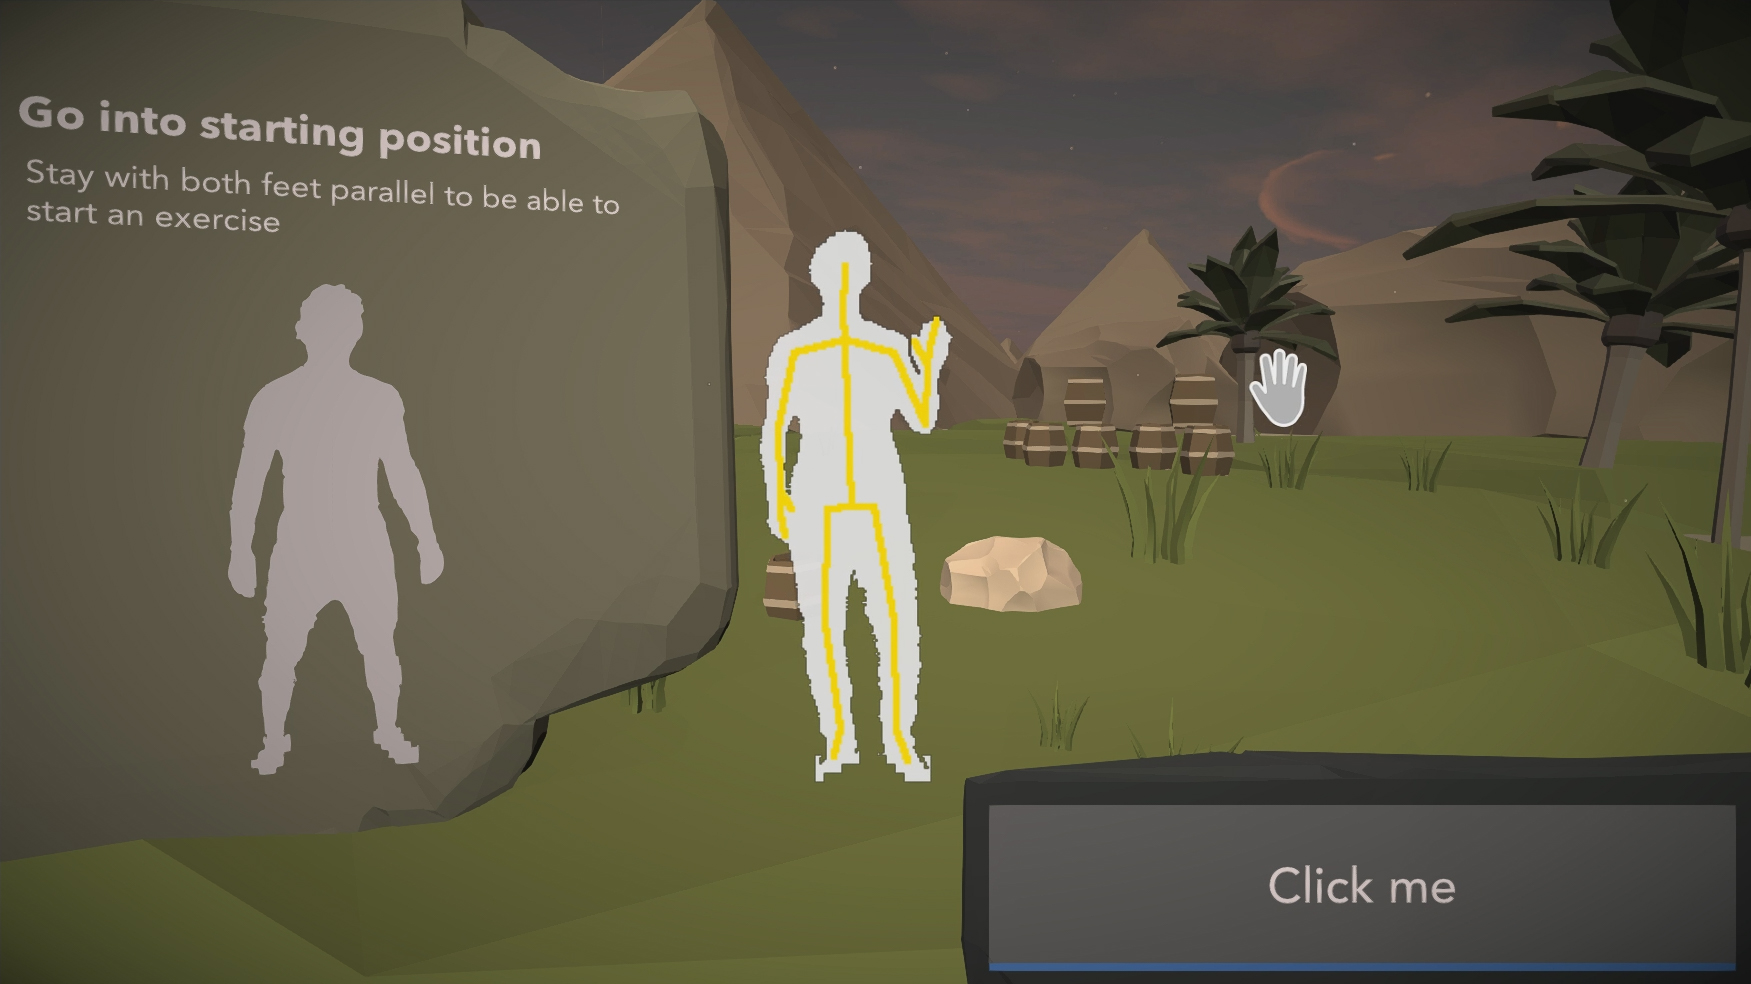
\includegraphics[width=0.5\linewidth]{Pictures/5_Workflow/4_2_StartingPosition}
	\caption{Instruction on how to use stand in the correct position}
	\label{fig:5_3_standingPosition}
\end{figure}

\subsubsection{Selection Menus}
The system consists of several selection menus. At first a user profile has to be selected (Figure~\ref{fig:5_3_user_menu}). Hereby it provides the possibility that more than one user can train with the system separately.
%When the trainee selects her profile the system checks if the JSON file has any data. If no data is available, which means it is a new user, the default exercise JSON file will be copied into the profile. 
When selecting a profile the appropriate JSON file will be loaded into the system for accessing and managing the user data.
%The trainee selects her profile by herself. With this the data will be loaded into the system. In the user selection the trainee should select the right profile by herself to cover the condition of multiple user that can train with the system. 
%The users name and id are saved in as \textit{PlayerPrefs}. This is a class in Unity that provides the possibility to be globally accessible in the application. The respective code for setting and getting the values can be seen in listing \todo{ref listing playerpfrefs}. This is needed to find the correct path for the JSON files to save the data.

Levels and exercises are also structured as menu (Figure~\ref{fig:5_3_level_menu} \&~\ref{fig:5_3_exercise_menu}).
At first they are all locked except the very first one to provide a starting point.
A level can be unlocked by accomplishing each exercise of the previous level.
This procedure applies similarly to the exercises.
Hereby, the next exercise can be unlocked by accomplishing all body sides and repetitions of the current exercise.
%The structure already seen in section \textit{\ref{4_4_exercises}} is adapted to store the corresponding information for the tier, exercise, side, and repetition.
\begin{figure}[htb]
	\centering
	\begin{minipage}[t]{0.32\linewidth}
		\centering
		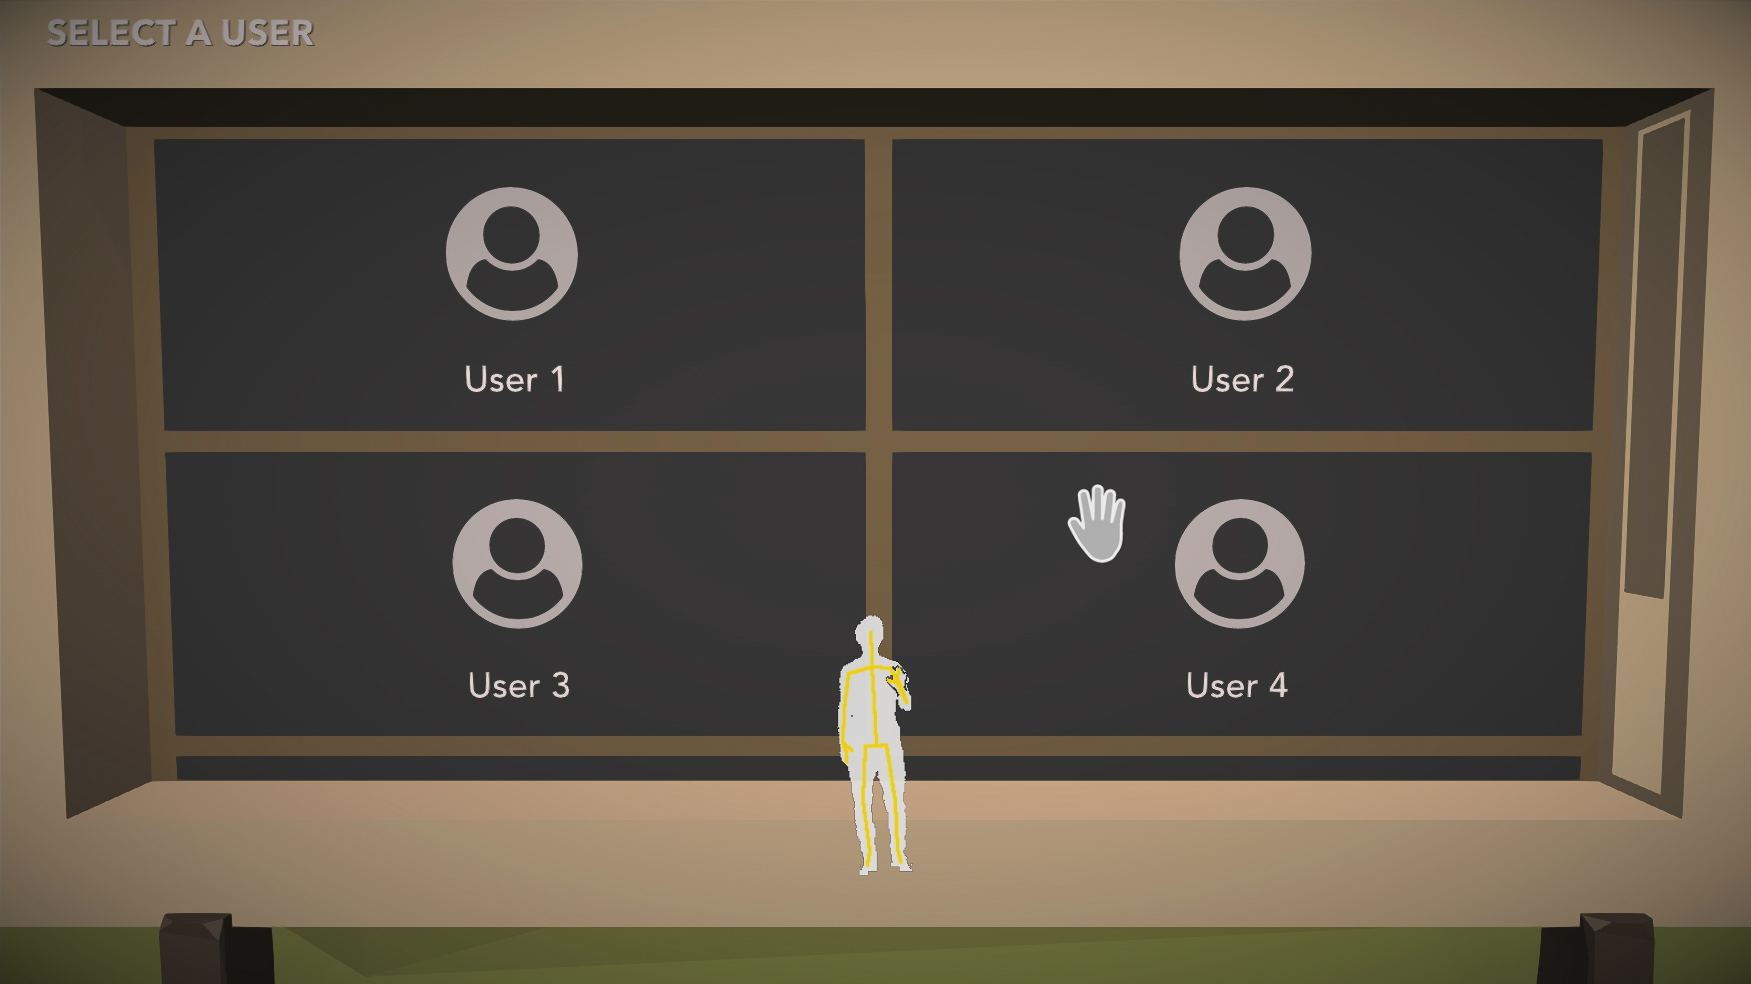
\includegraphics[width=1\linewidth]{Pictures/5_Workflow/5_UserMenu}
		\subcaption{User menu}%
		\label{fig:5_3_user_menu}
	\end{minipage}
	\hfill
	\begin{minipage}[t]{0.32\linewidth}
		\centering
		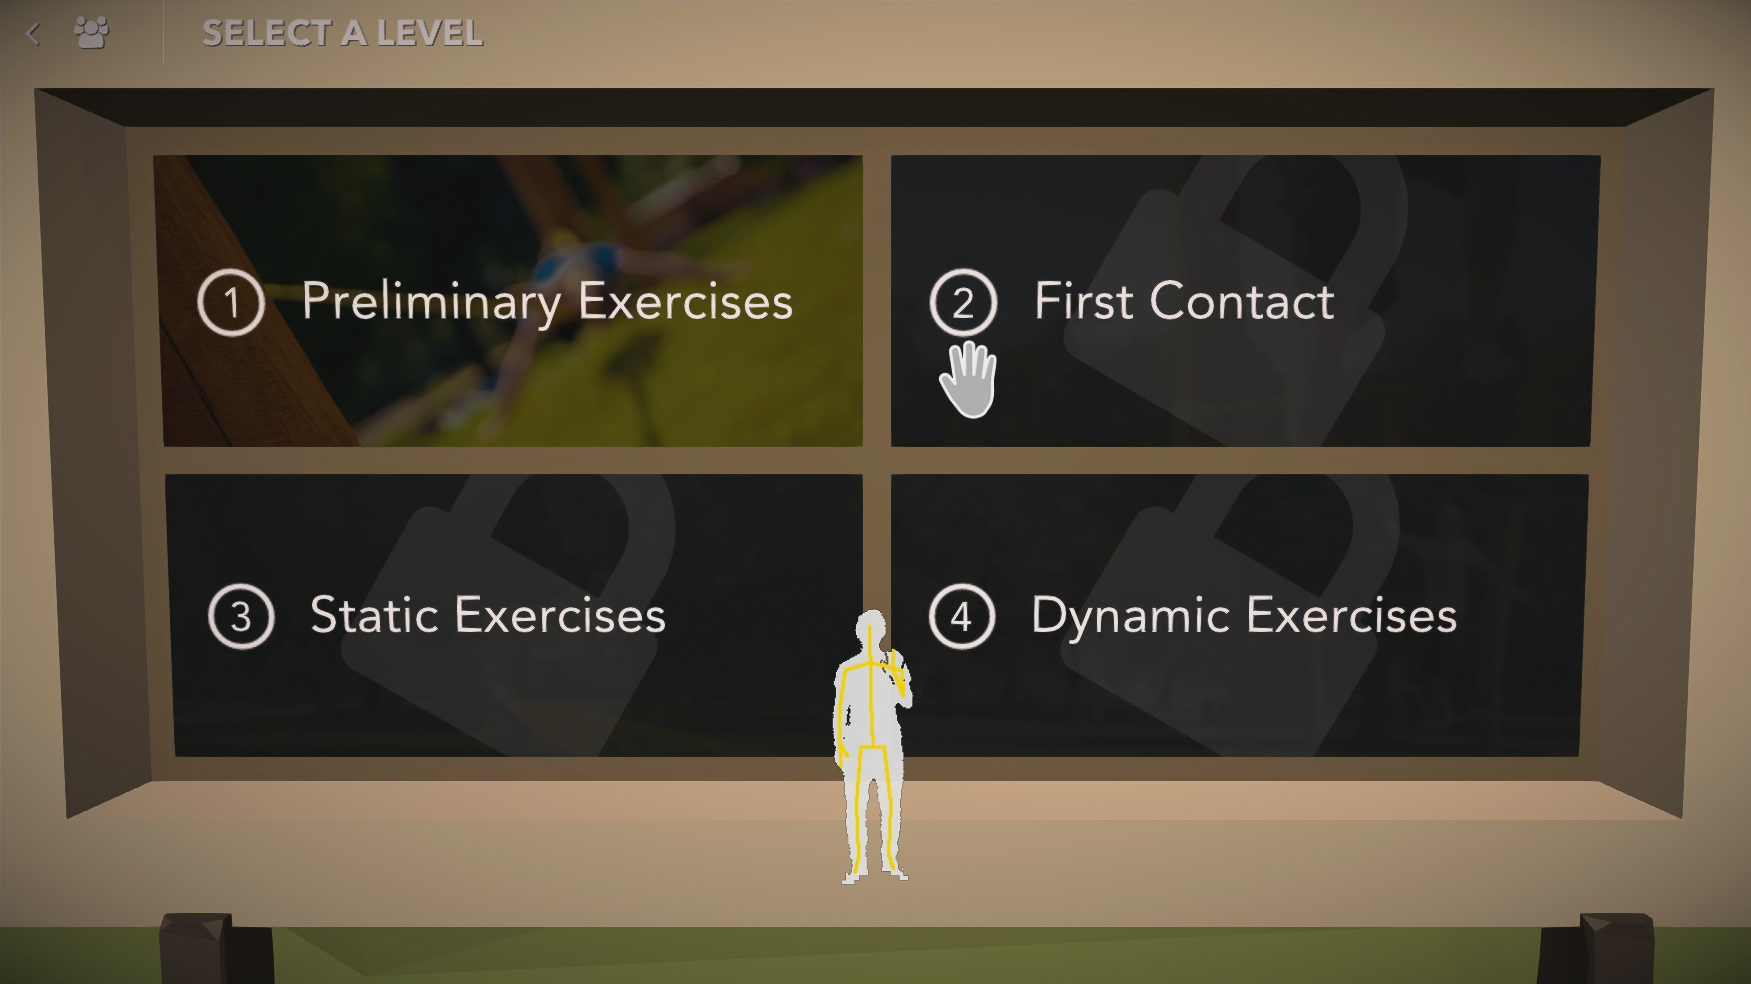
\includegraphics[width=1\linewidth]{Pictures/5_Workflow/6_LevelMenu}
		\subcaption{Level menu}%
		\label{fig:5_3_level_menu}
	\end{minipage}
	\hfill
	\begin{minipage}[t]{0.32\linewidth}
		\centering
		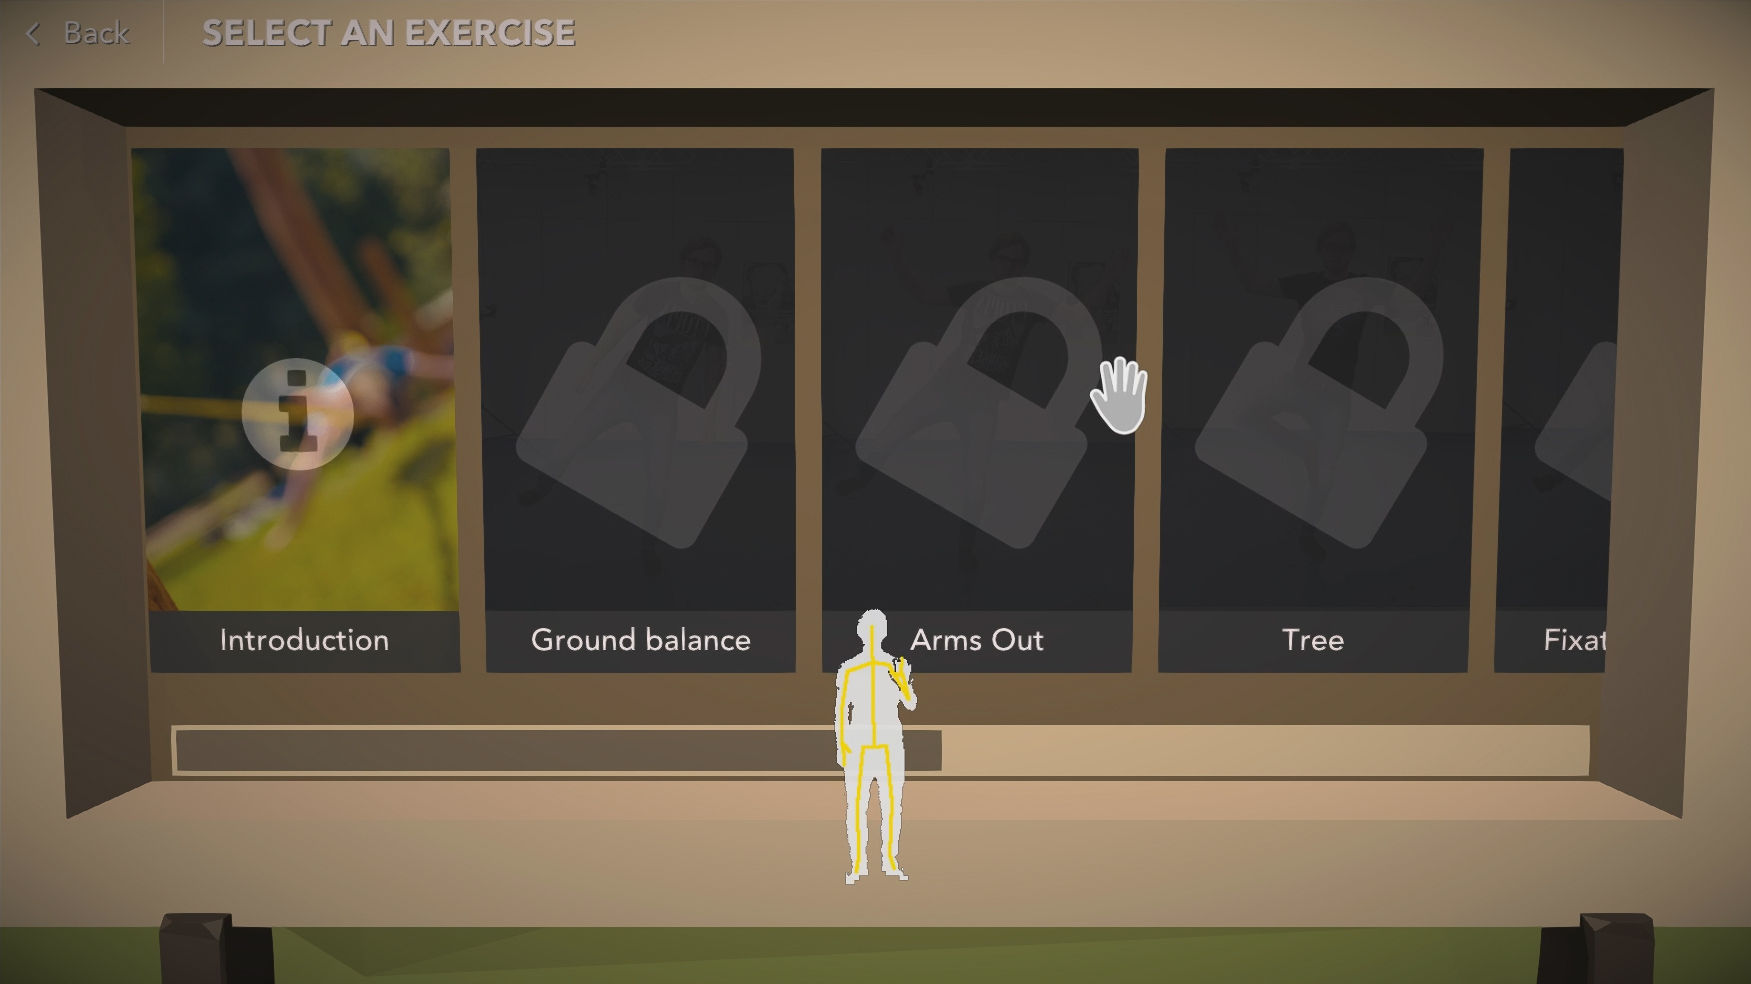
\includegraphics[width=1\linewidth]{Pictures/5_Workflow/7_1_ExerciseMenu}
		\subcaption{Exercise menu}%
		\label{fig:5_3_exercise_menu}
	\end{minipage}
	\caption{Visualisation of selection menus}%
	\label{fig:5_3_selection_menus}
\end{figure}

\subsubsection{Level and Exercise Description}
Selecting a level leads the user to the level introduction (Figure~\ref{fig:5_3_level_intro}). She is informed about the goals of the current level and gets helpful information for the execution of the following exercises. After that she selects the first exercise in the menu and afterwards a body side, which she wants to train first (Figure~\ref{fig:5_3_select_side}). This leads her to the detailed exercise description (Figure~\ref{fig:5_3_exercise_intro}). It is introduced by a list of actions she has to follow to perform it correctly. Additionally, the amount of repetitions and the minimum time to hold the gesture are given. Furthermore, a looping video on the visualizes the correct execution to the user.
\begin{figure}[htb]
	\centering
	\begin{minipage}[t]{0.32\linewidth}
		\centering
		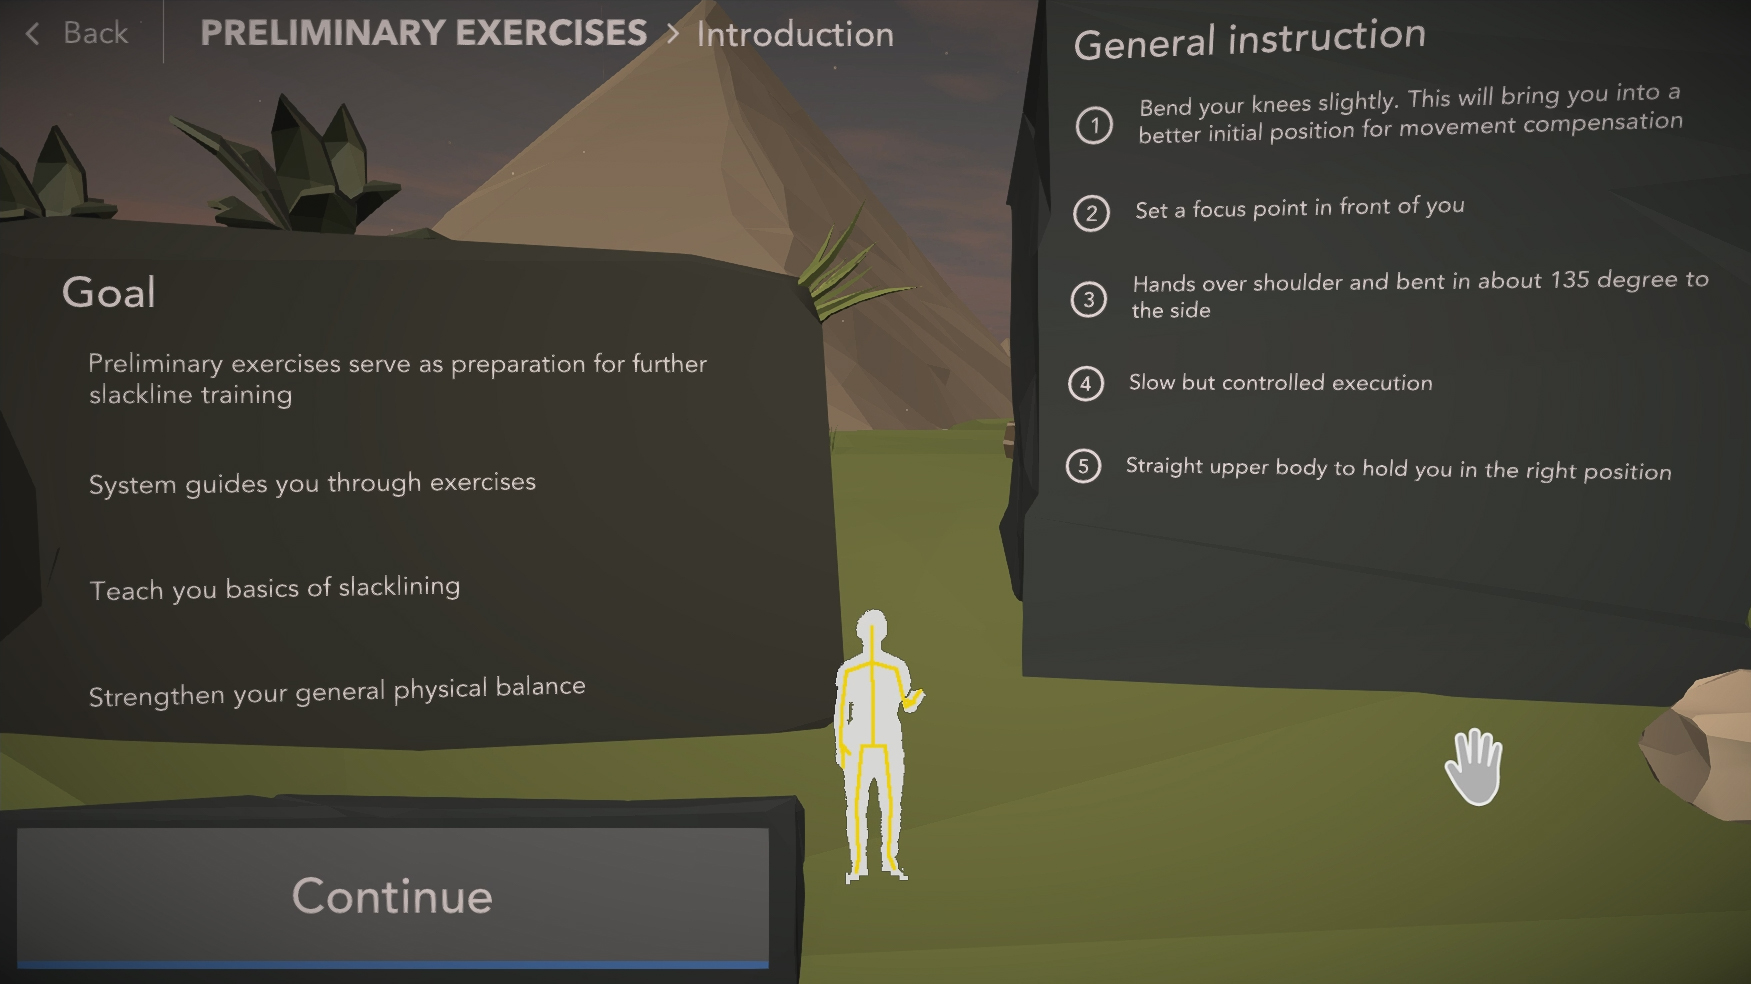
\includegraphics[width=1\linewidth]{Pictures/5_Workflow/8_LevelDescription}
		\subcaption{Goals \& tips for a level}%
		\label{fig:5_3_level_intro}
	\end{minipage}
	\hfill
	\begin{minipage}[t]{0.32\linewidth}
		\centering
		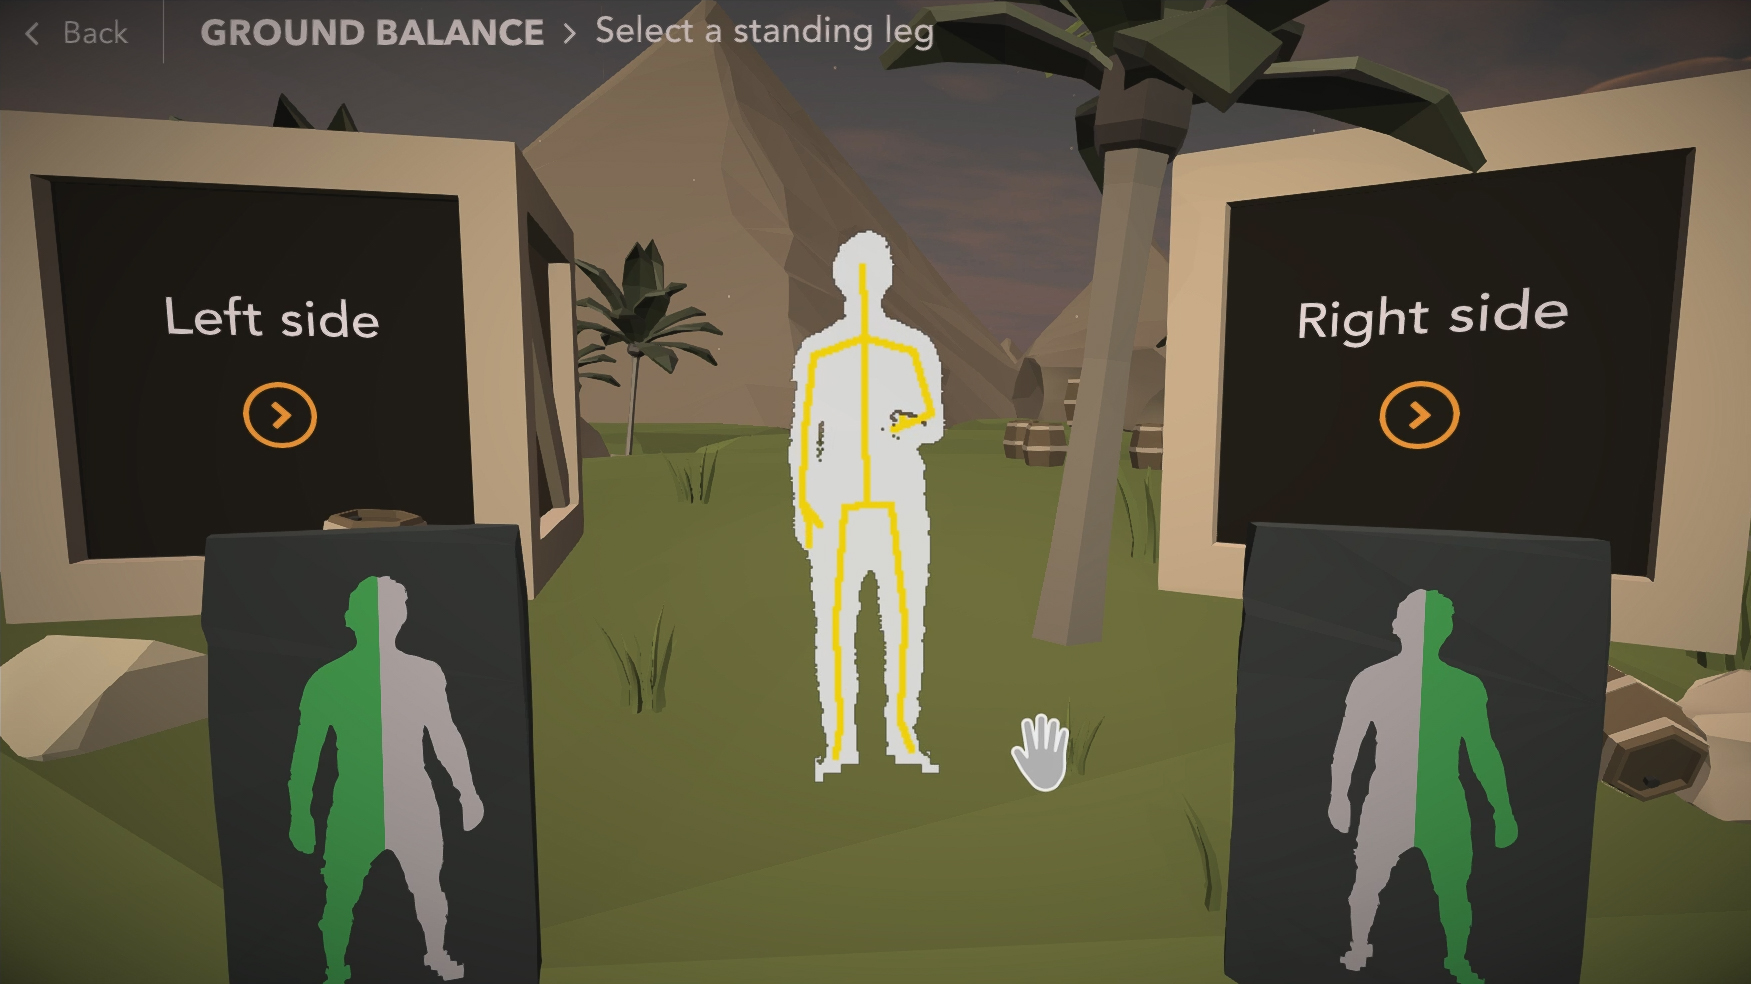
\includegraphics[width=1\linewidth]{Pictures/5_Workflow/9_1_SideSelectionNone}
		\subcaption{Selection of a body side}%
		\label{fig:5_3_select_side}
	\end{minipage}
	\hfill
	\begin{minipage}[t]{0.32\linewidth}
		\centering
		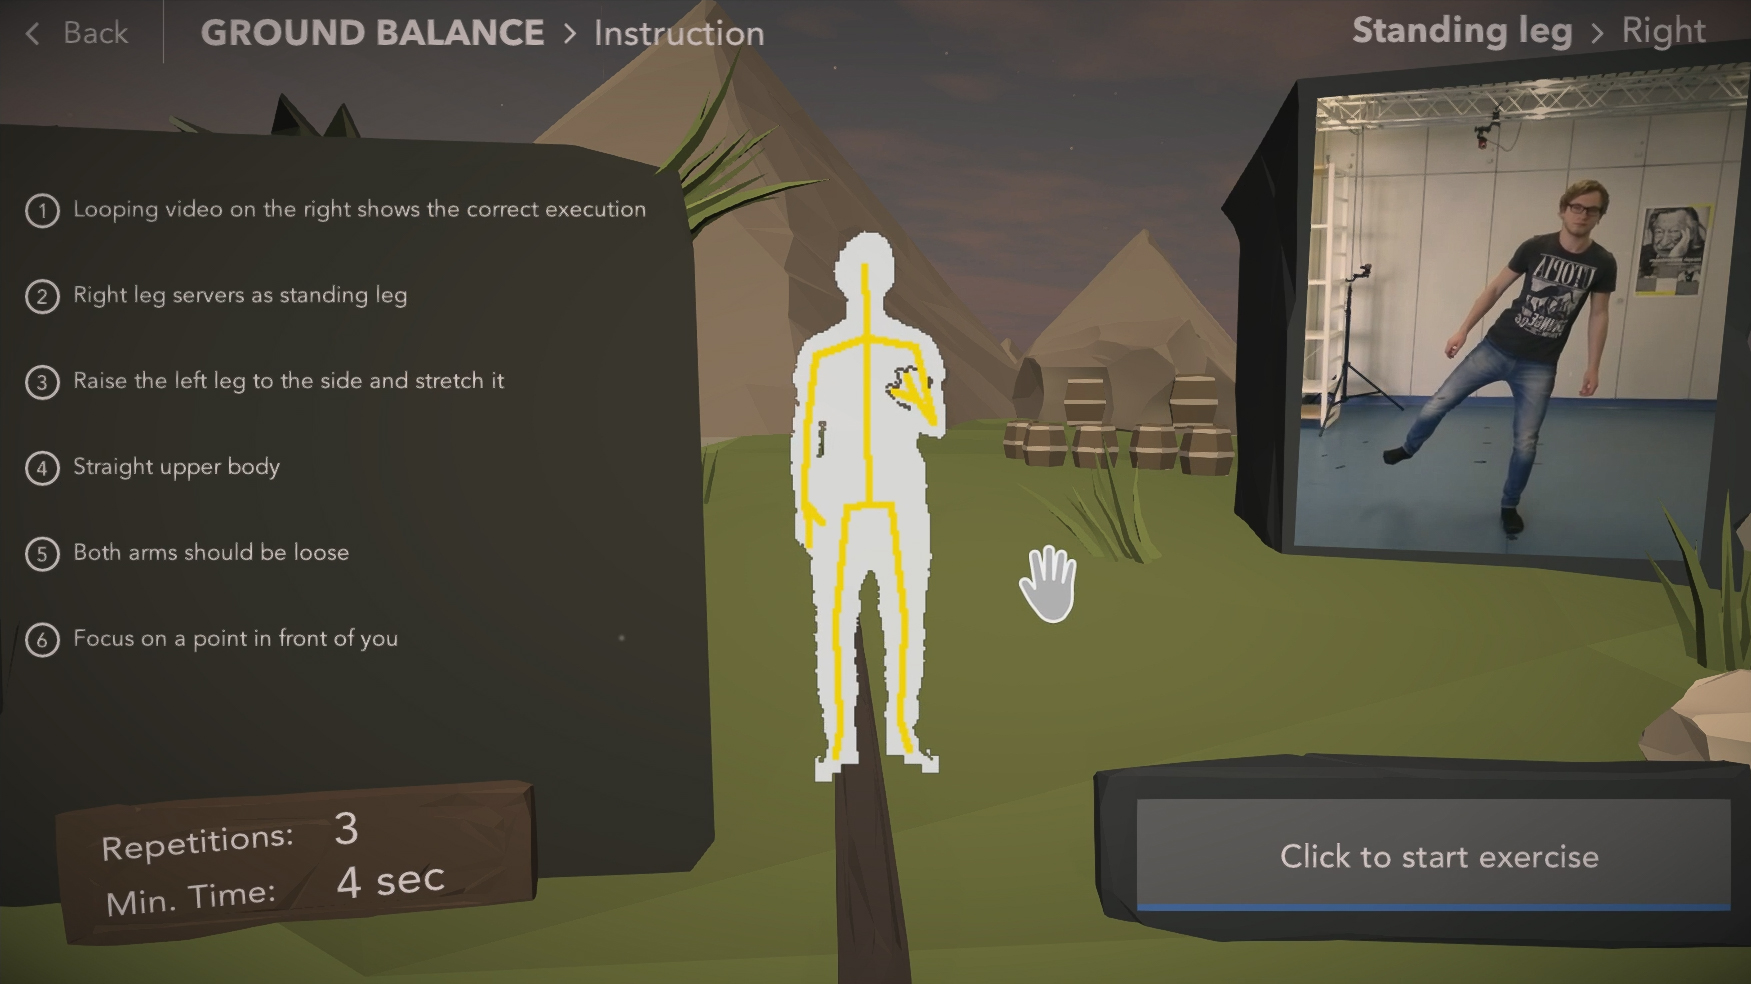
\includegraphics[width=1\linewidth]{Pictures/5_Workflow/10_ExerciseInstruction}
		\subcaption{Instruction into an exercise}%
		\label{fig:5_3_exercise_intro}
	\end{minipage}
	\caption{Instruction screens for a level and an exercises}%
	\label{fig:5_3_introductions}
\end{figure}

\subsubsection{Exercise Execution}
The exercise execution consists of the biggest functionality implementation (Figure~\ref{fig:5_3_exercise_execution}). Feedback indicators provide the user with necessary information about the current exercise in real time. This should help to enhance the performance in her execution and for successfully accomplishing the exercise. In the SLS the following feedback indicators are integrated:

\begin{itemize}
\item Checklist about key elements of an exercise
\item Amount of repetitions in general, finished, and left
\item Correct performance of an exercise (Timer starts and confidence increases)
\item Elapsed time the user is performing the exercise (Timer with a filling circle)
\item How good the exercise is currently performed (Confidence/Progress bar)
\item If a repetition was successful (Audio signal, timer color, success text, and incrementing repetitions counter)
\item If a repetition attempt was not successful (Audio signal and timer reset)
\end{itemize}

\begin{comment}
\begin{itemize}
\item Checklist about key elements of an exercise (Small red cross if not in correct position or green checkmark if in correct position)
\item Amount of repetitions in general, finished, and left
\item Correct performance of an exercise (Timer starts and confidence begins to increase)
\item Elapsed time the user is performing the exercise (Big timer with a filling circle around it)
\item How good or far the exercise is currently performed (Blue confidence/progress bar)
\item If the repetition was successful (Audio signal, timer changes color to green, success text, and incrementing repetitions counter)
\item If a repetition attempt was not successful (Audio signal and timer reset)
\end{itemize}

\end{comment}

After each successful exercise execution the user is forwarded to a summary screen (Figure~\ref{fig:5_3_exercise_summary}).
She gets an overview about performance parameters for the execution time, attempts, and the confidence for each repetition. Averaged values for the accomplished side summarize this.
%A similar summary screen exists for the entire level if all exercises of it have been accomplished. The same parameters are given but averaged (Figure~\ref{fig:5_3_level_summary}).
A similar summary screen for the entire level can be selected in the exercise menu. It provides an overview of the same performance parameters for each exercise in average (Figure~\ref{fig:5_3_level_summary}).

\begin{comment}
\item When an exercise is currently correctly performed
\item How good the exercise is currently performed, namely the confidence
\item The elapsed time the user is performing the exercise
\item When the repetition is successfully accomplished, i.e. the minimum time has been reached
\item When an repetition attempt was not successful
\item How many repetitions in general, finished and left
\item Checklist about key elements in an execution (like hands up, foot stretched, etc.)
\item A summary that shows the user parameters about the performance (execution time, overall attempts, confidence) for each repetition and an average value of these
\item A similar summary can also be found for the entire stage, where the same parameters for each exercise are listed in average
\end{comment}

\begin{figure}[htb]
	\centering
	\begin{minipage}[t]{1\linewidth}
		\centering
		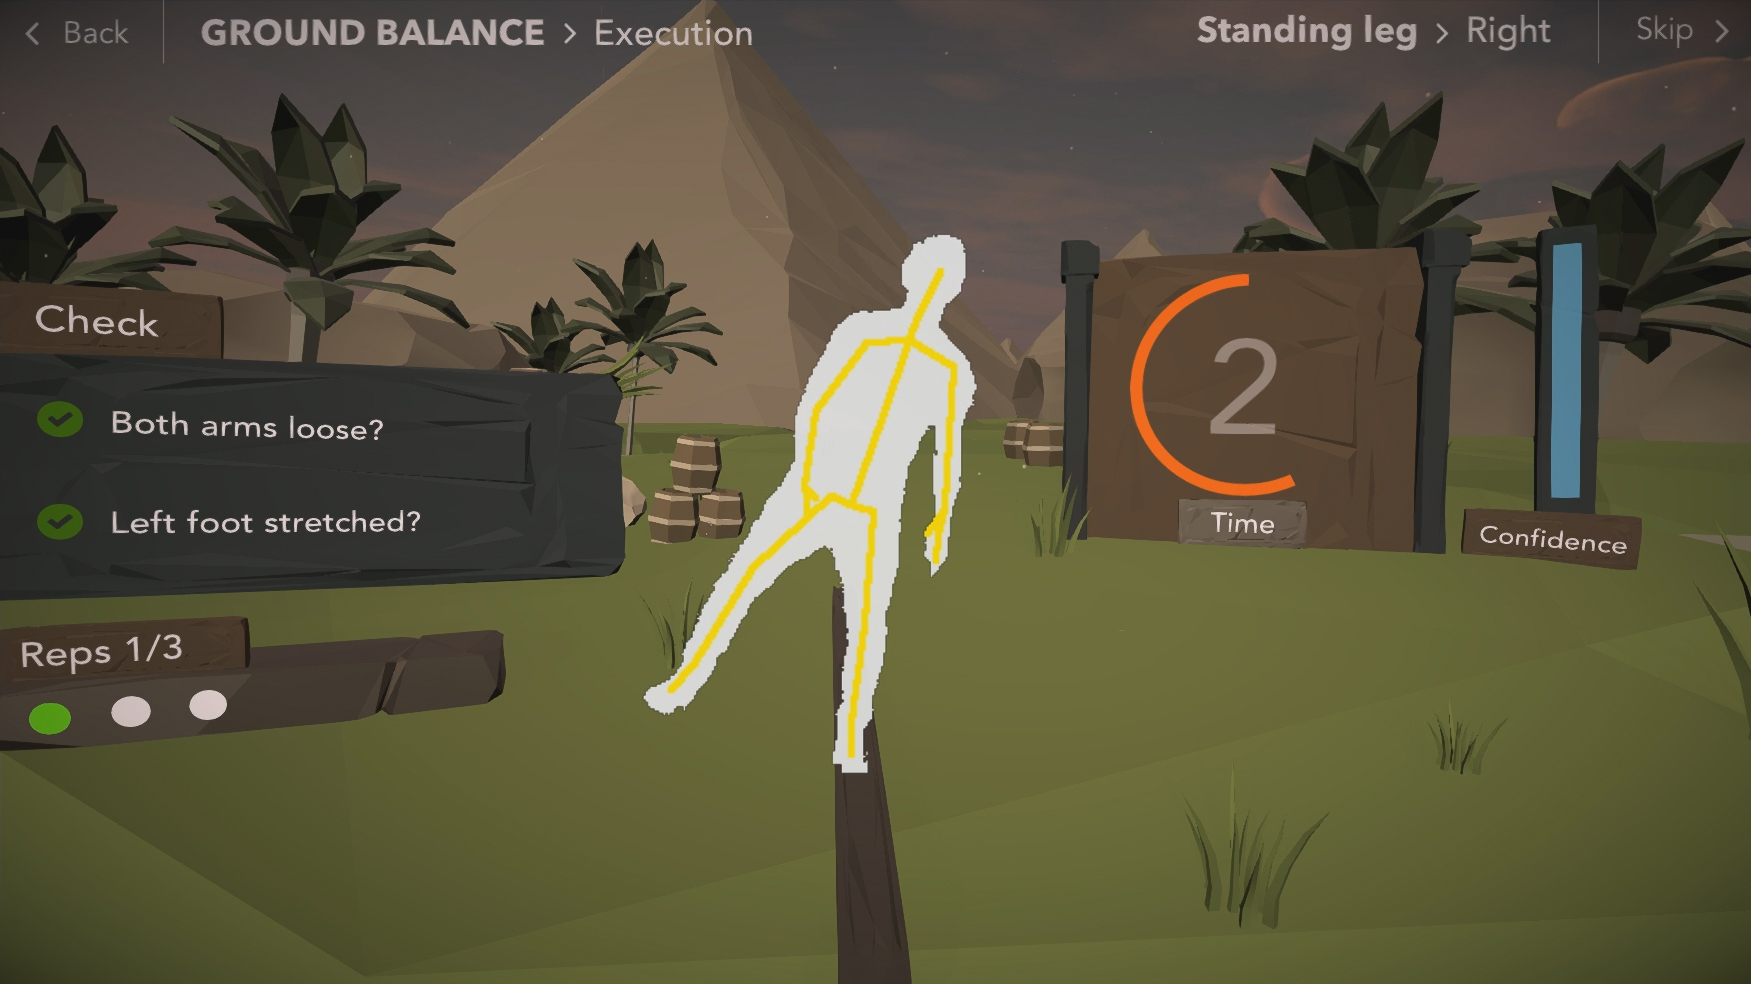
\includegraphics[width=0.57\linewidth]{Pictures/5_Workflow/11_3_ExerciseExecutionRep}
		\subcaption{Exercise execution}
		\label{fig:5_3_exercise_execution}
	\end{minipage}
	\hfill
	\begin{minipage}[t]{0.49\linewidth}
		\centering
		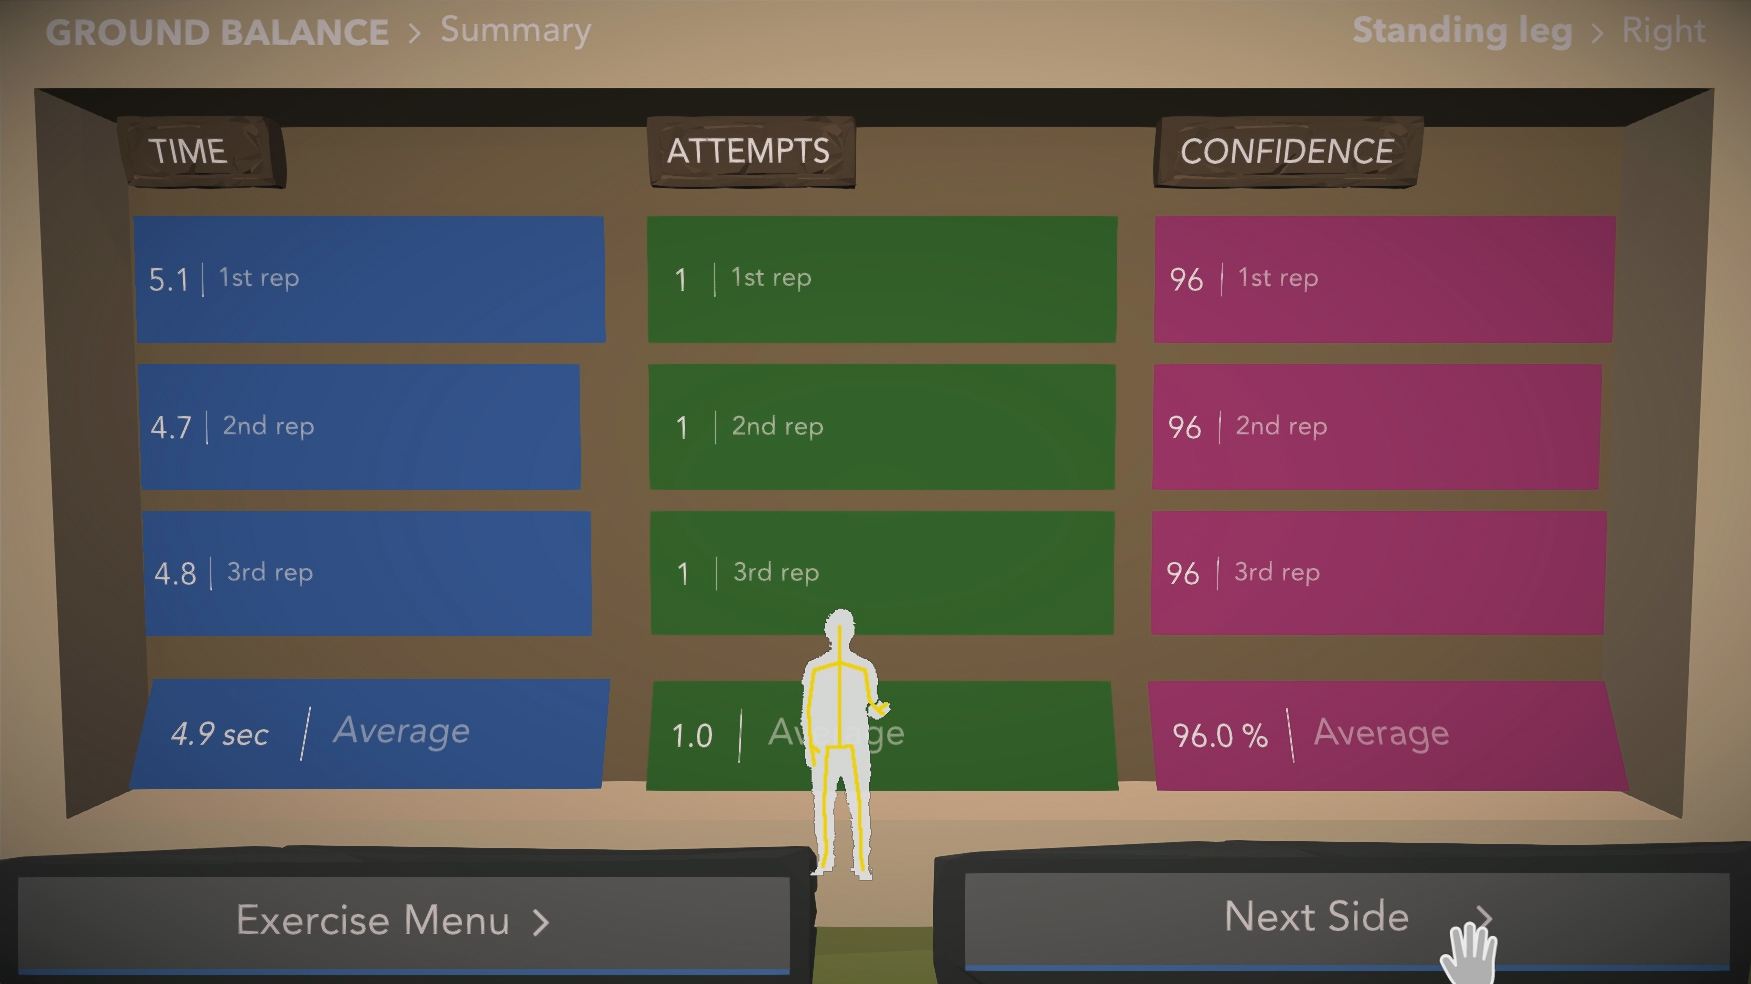
\includegraphics[width=1\linewidth]{Pictures/5_Workflow/12_ExerciseSummary}
		\subcaption{Exercise summary}
		\label{fig:5_3_exercise_summary}
	\end{minipage}
	\hfill
	\begin{minipage}[t]{0.49\linewidth}
		\centering
		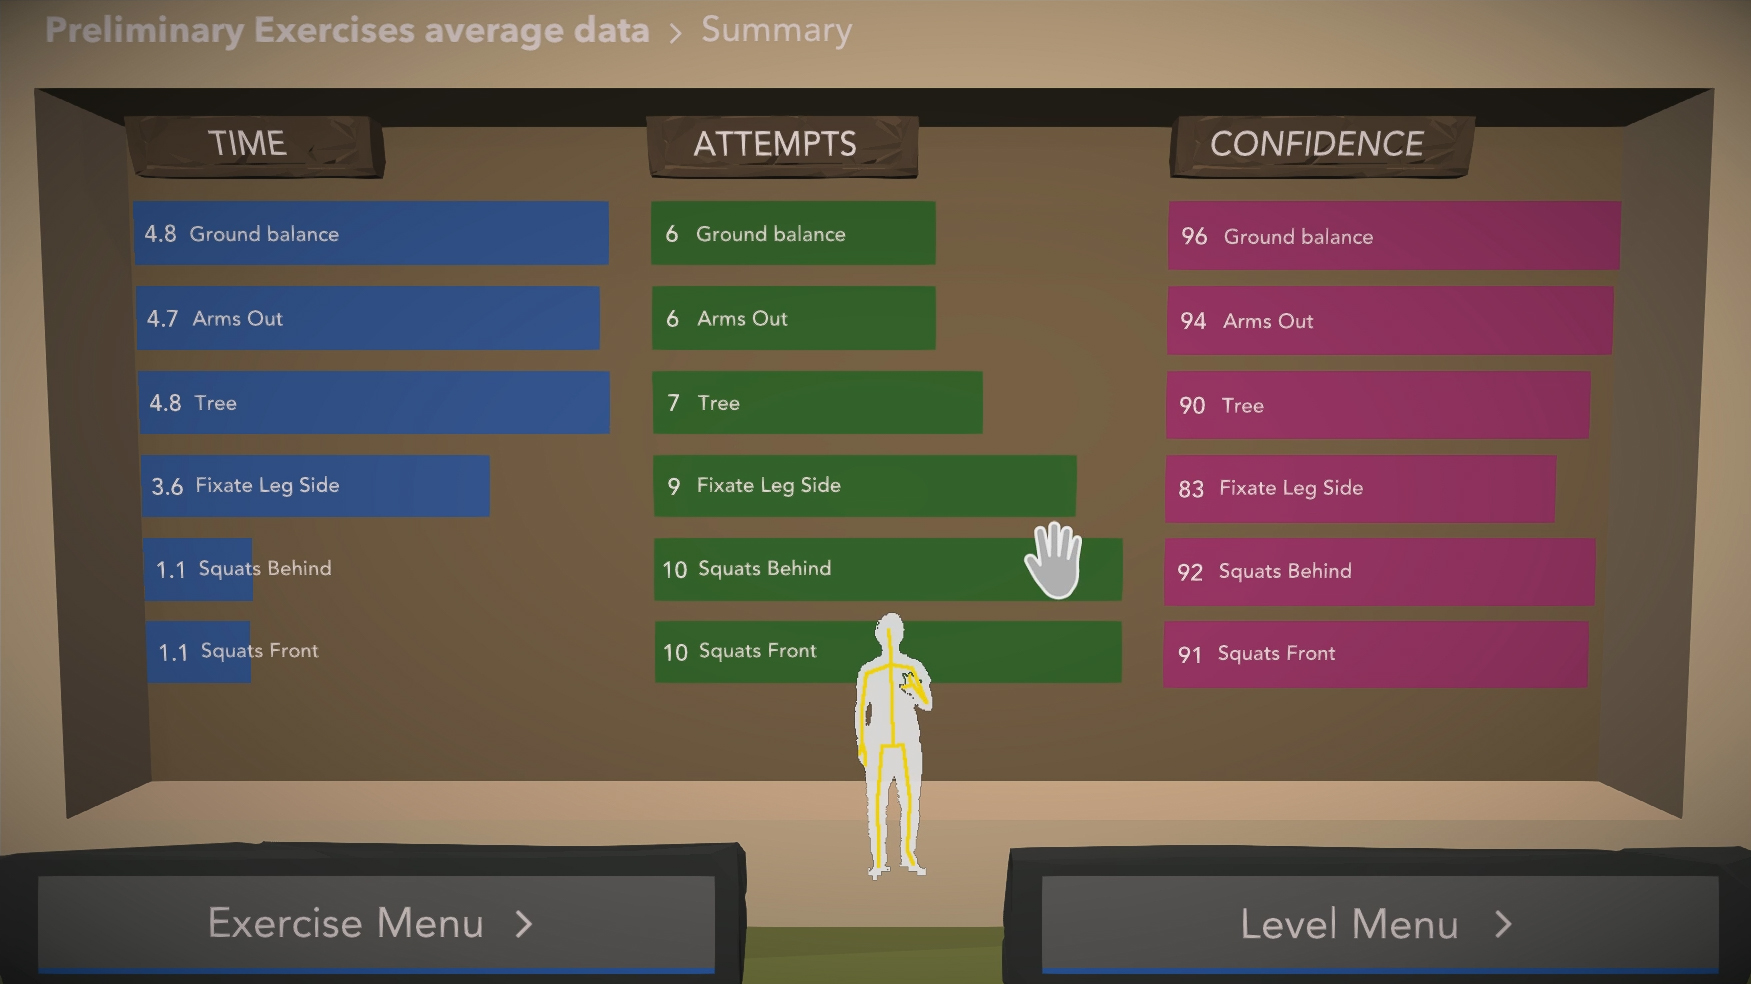
\includegraphics[width=1\linewidth]{Pictures/5_Workflow/13_TierSummary}
		\subcaption{Level summary}
		\label{fig:5_3_level_summary}
	\end{minipage}
	\caption{Exercise execution and summary screens}
	\label{fig:5_3_exercise_sequence}
\end{figure}


\begin{comment}
- Kinect used for tracking --> how Kinect tracks user - skeleton, infrared, own algorithm -> RW

- Technical feasibility in here?

- Recording of gestures --> Kinectstudio --> Making/Train gestures --> Visual gestures builder

- System architecture of system --> Unity3D, Kinect SDK, Kinectstudio, VGB --> kinect sdk free to use since version X

- Data management --> json file, default exercise json and each user has its own json file 

- Engagement with Kinect

- Interaction components (track hand joints, PHIZ, Constraints) --> different interactions tested (closing hand, V-sign, hover, pushing) --> not all good because of distance to Kinect --> In unity addon written for managing data --> create new users, load exercise in user, adjust jsons

- tier and exercises as level design --> locked and unlocking by successfully accomplishing exercise

- Integration VGB databases in Unity and how to track gestures in it --> gesturedetector, eventlistener

- Providing feedback properly --> confidence/progress of gestures in event listener, checklist (joint detection), 
--> user viewer --> how it works (making cloudy map regarding user position, drawing lines for skeletons)

- Summary screen --> feedback about prior or entire tier performance with time, confidence and attempts

- User interface design --> sketches, mock ups, development --> workflow figure
\end{comment}

\section{User Interface}\label{5_4_userInterface}
The user starts with an engagement gesture which is implemented as raising her hand over the head. After that a tutorial about interaction techniques of the system will be given. Now that she's confident with the system interaction she can select her profile in the user menu. This loads the profile which leads further to the level selection menu. In here she can select a level, whereas initially the first one is can be selected. Selecting a level leads to the exercise menu. In here she has to read initially the stage introduction to become a basic understanding about the exercises within. After reading this, it unlocks the first exercise. Selecting an exercise leads to the side selection, where the user has to choose the side she wants to train. This is followed by an introduction of the exercise, in which is explained how to perform it correctly. If the user is ready, she should stay in a starting position to be able to start the exercise execution. Then she find herself in the exercise execution scene. It provides indicators to correctly execute the exercise, like the time, repetitions, confidence and a checklist. After finishing with the exercise, a summary is shown which summarizes the user performance. Then she can return to the main menu or directly try the next exercise. At the end of each stage an overall summary gives an overview about all exercises with average performance parameters.

The user should be introduced to the stage. In here the purpose, goal, and helpful techniques should be given, such that the user becomes an overview about the exercises. At last a summary scene shows several performance parameter for the exercises in this stage.

\begin{figure}[htb]
	\centering
	\begin{minipage}[t]{1\linewidth}
		\centering
		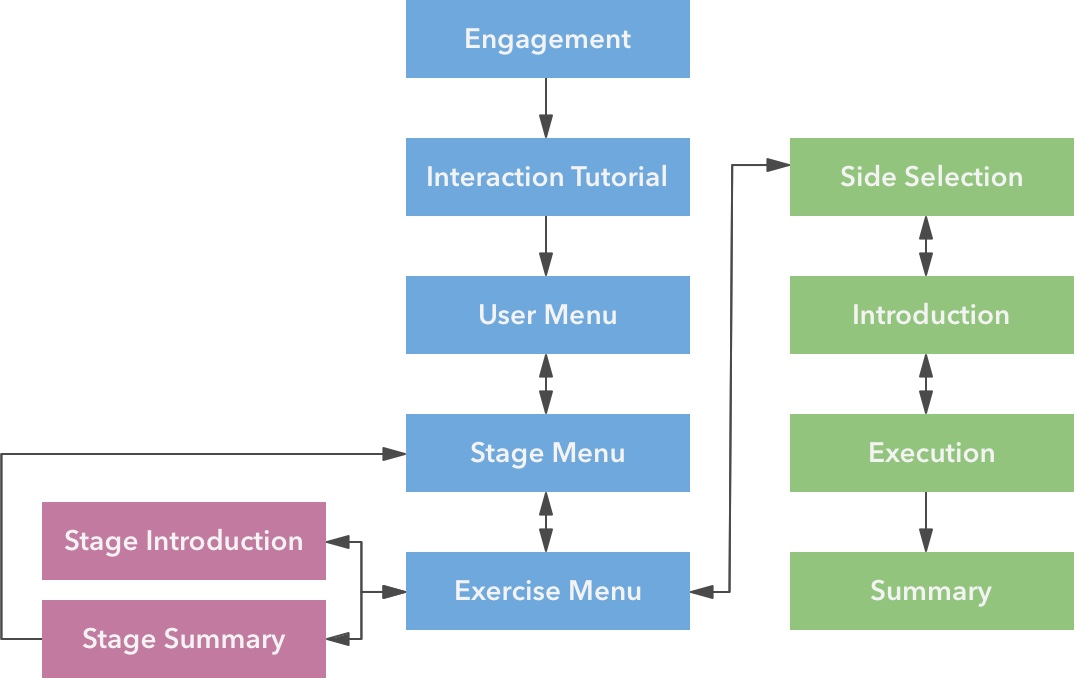
\includegraphics[width=1\linewidth]{Pictures/5_1_UIWorkflow}
		\caption{Scenario workflow}
		\label{fig:scenarioWorkflow}
	\end{minipage}
\end{figure}
